\begin{document}

\mode<presentation>{
\title{Introduction to Quantum Computing and Spin Networks}
\author{dln-dev}
\date{February 13th 2017}
%\logo{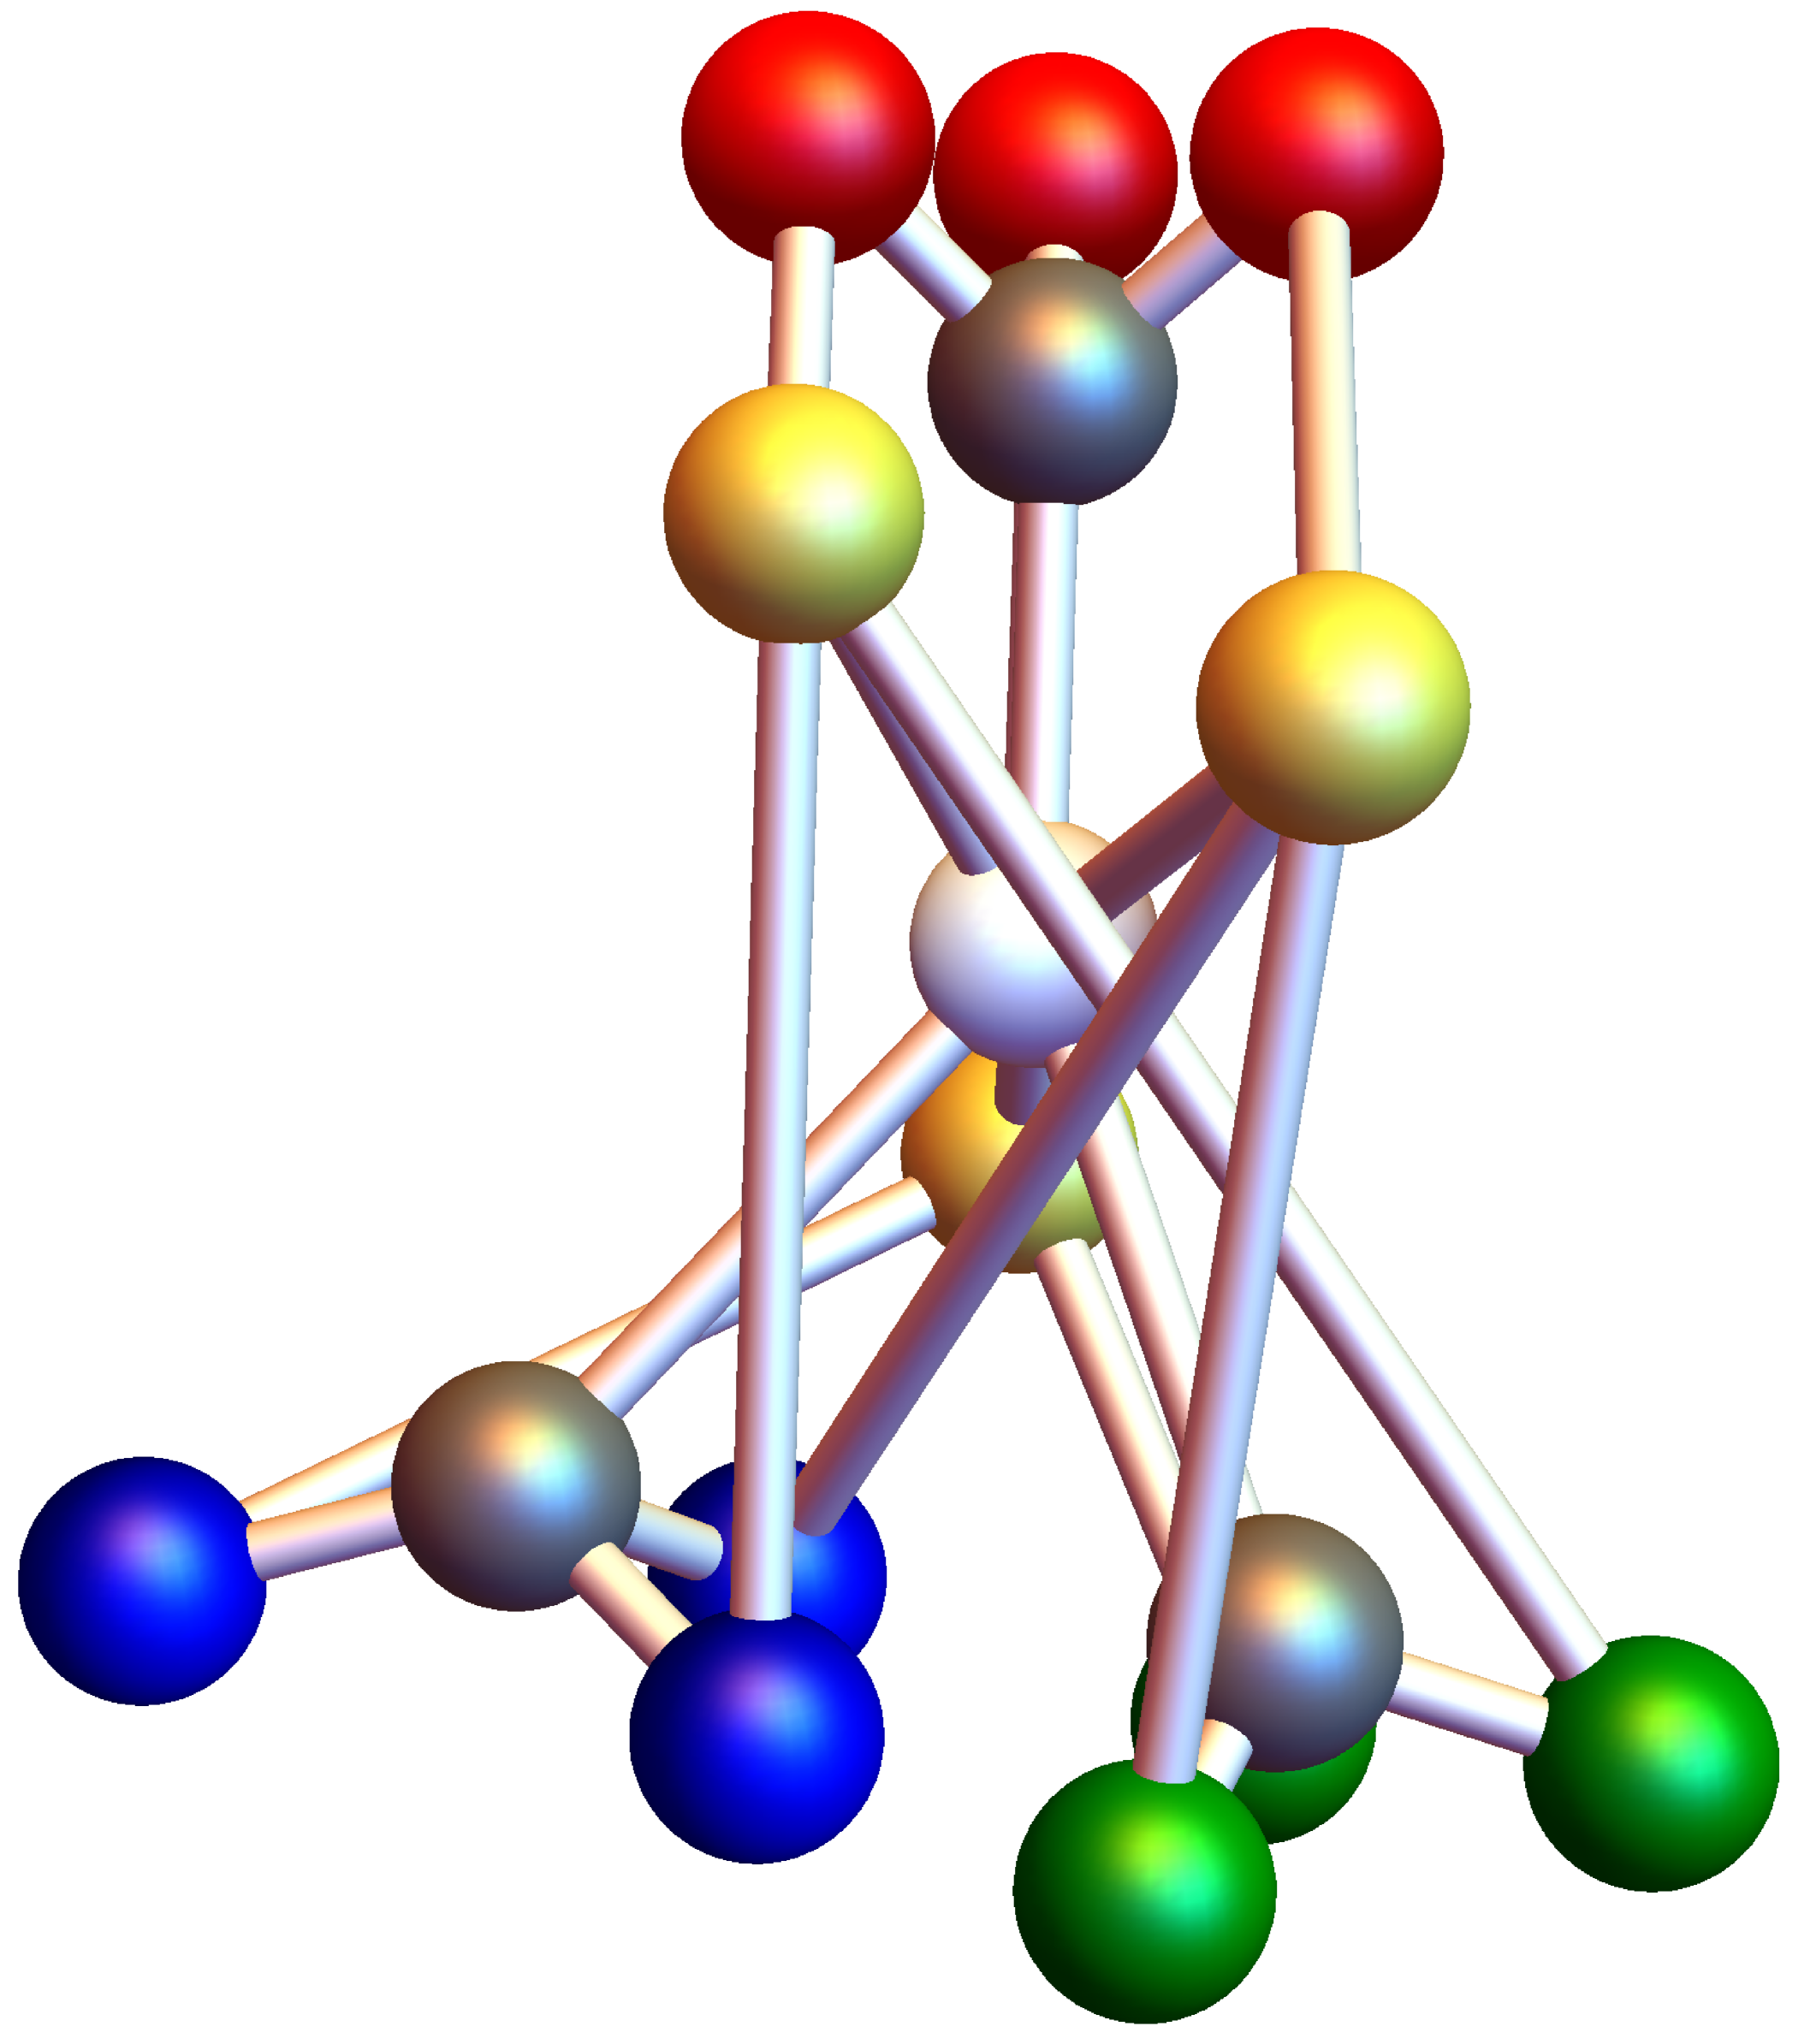
\includegraphics[width=\textwidth]{Images/switch_square}}
\titlegraphic{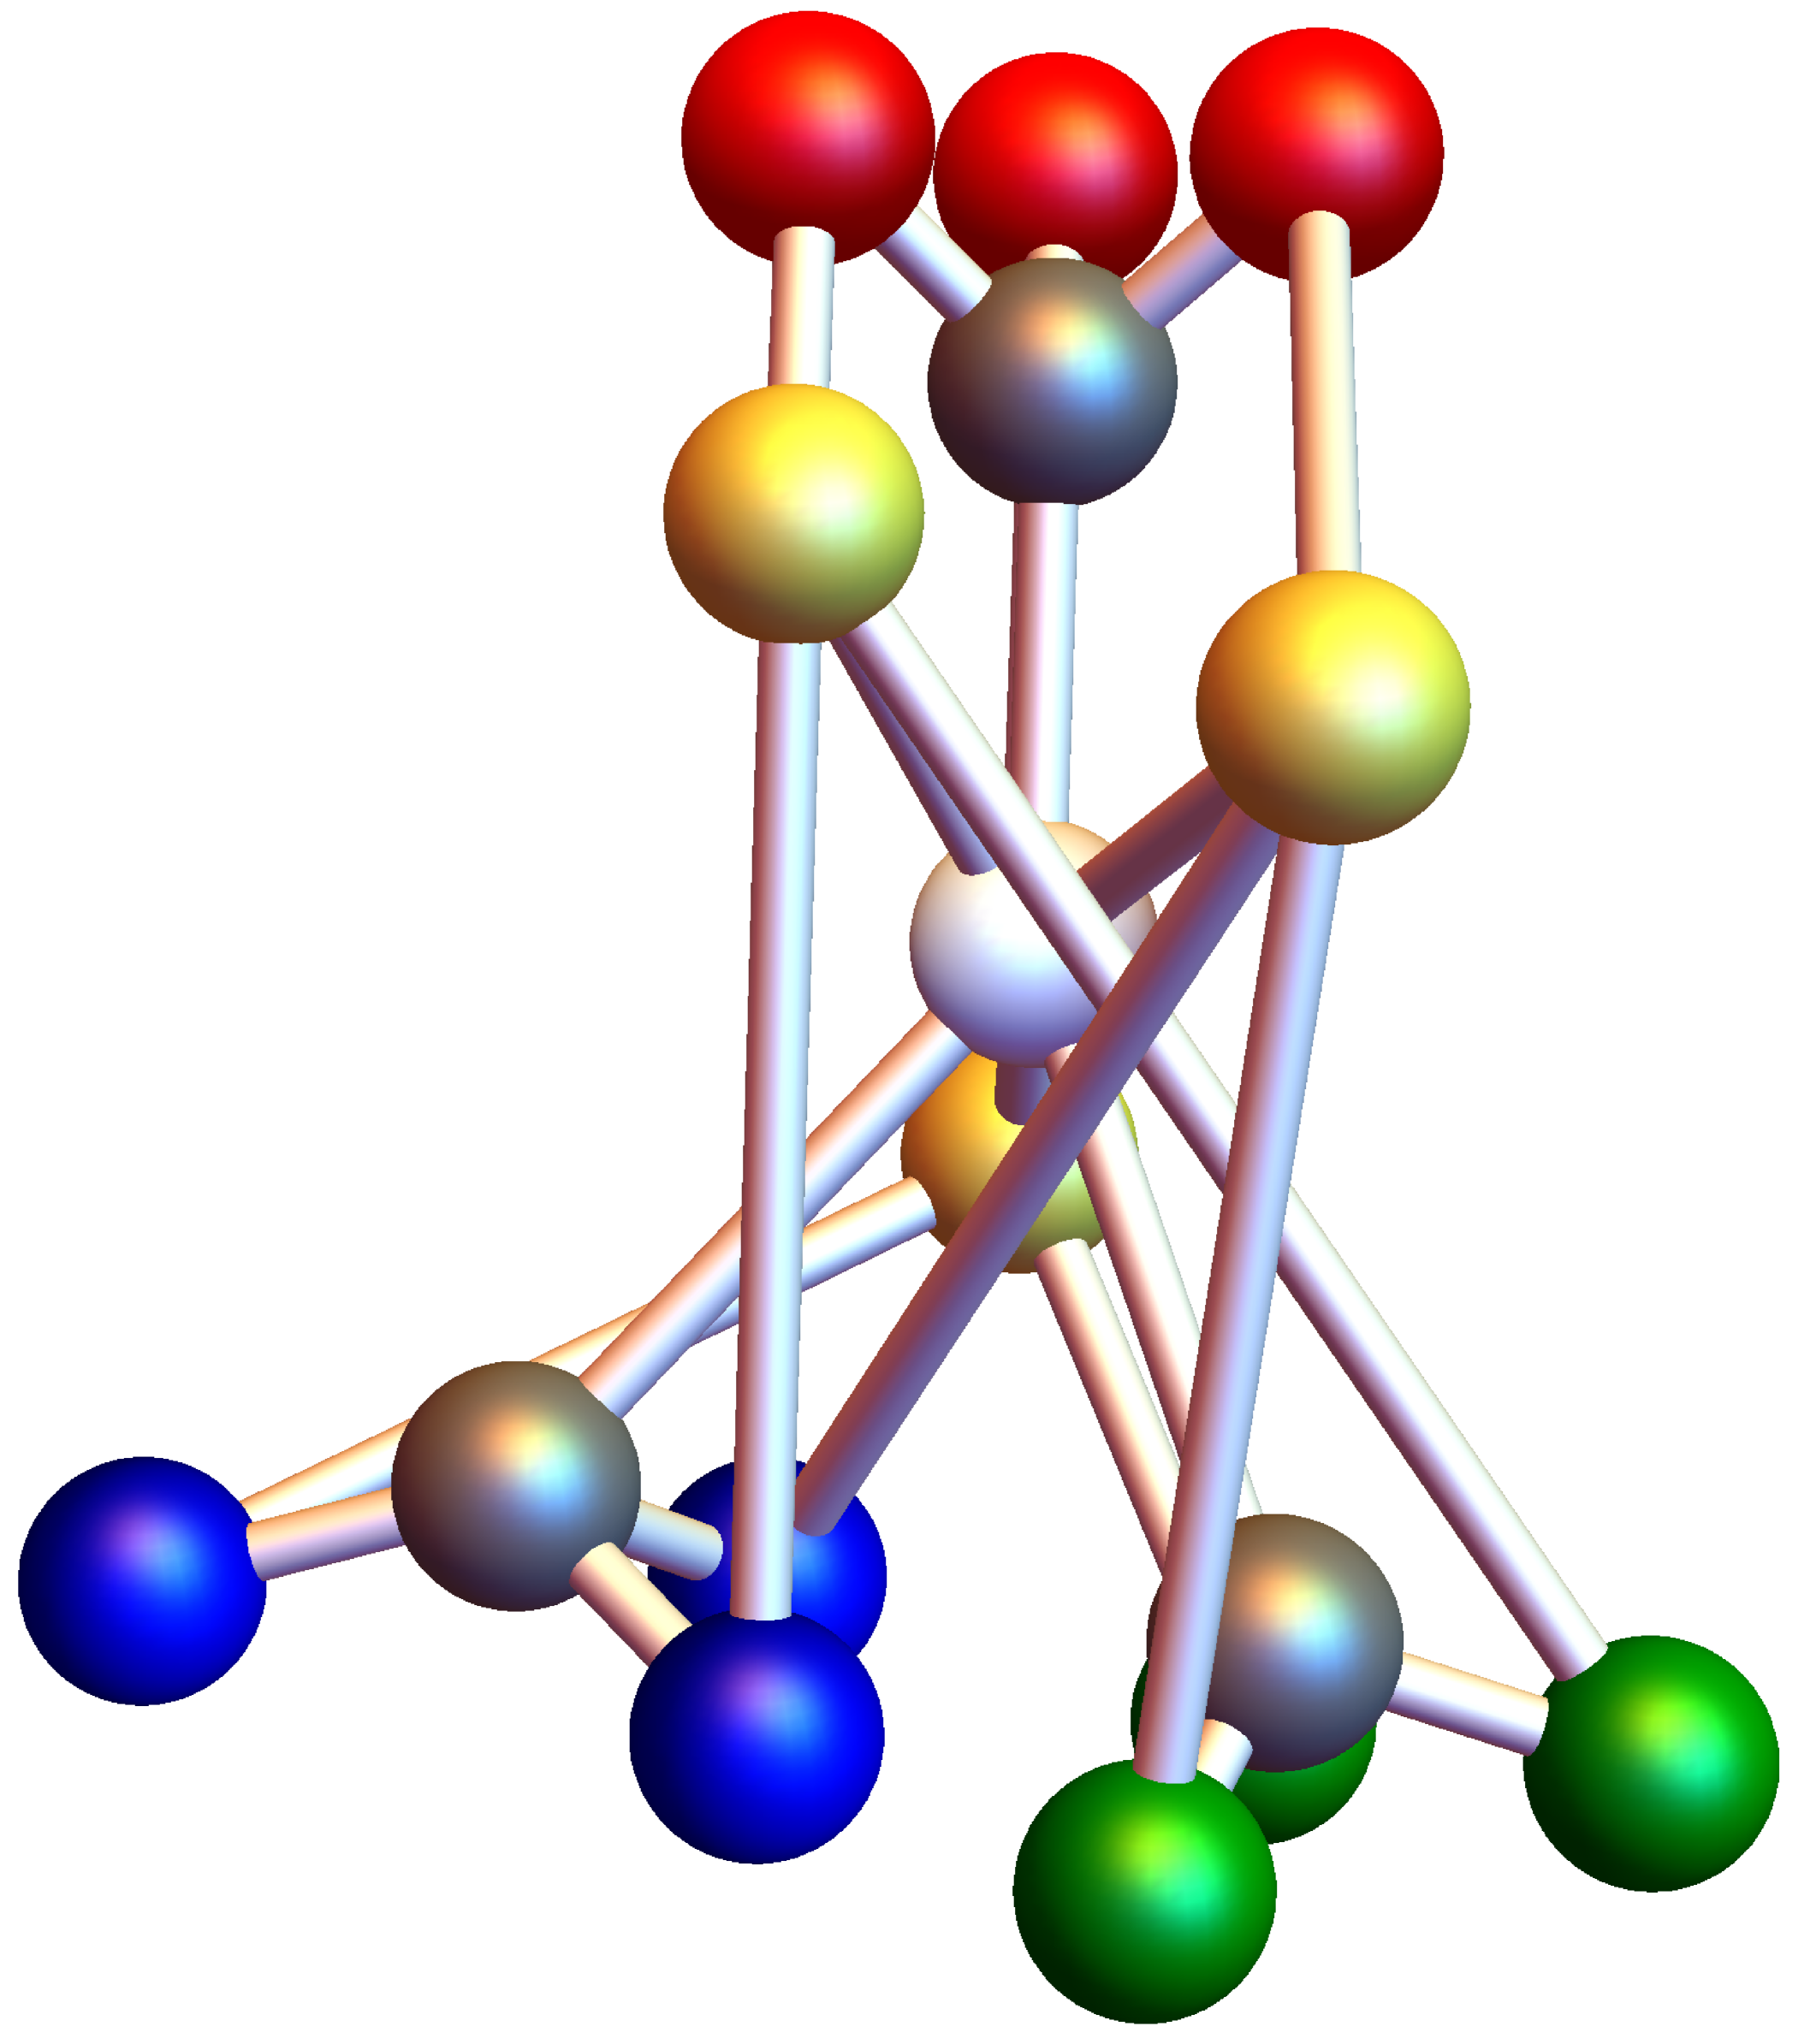
\includegraphics[width=0.1\textwidth]{Images/switch_square}}

\frame{\titlepage}
}

\mode<article>{\begin{titlepage}
	\center
	\vspace*{5.0cm}
	{ \huge \bfseries Introduction to Quantum Computing and Spin Networks}\\[0.4cm]

	\textsc{\Large dln-dev}\\[1.5cm]
	{\large February 13th 2017}\\[5.0cm]

	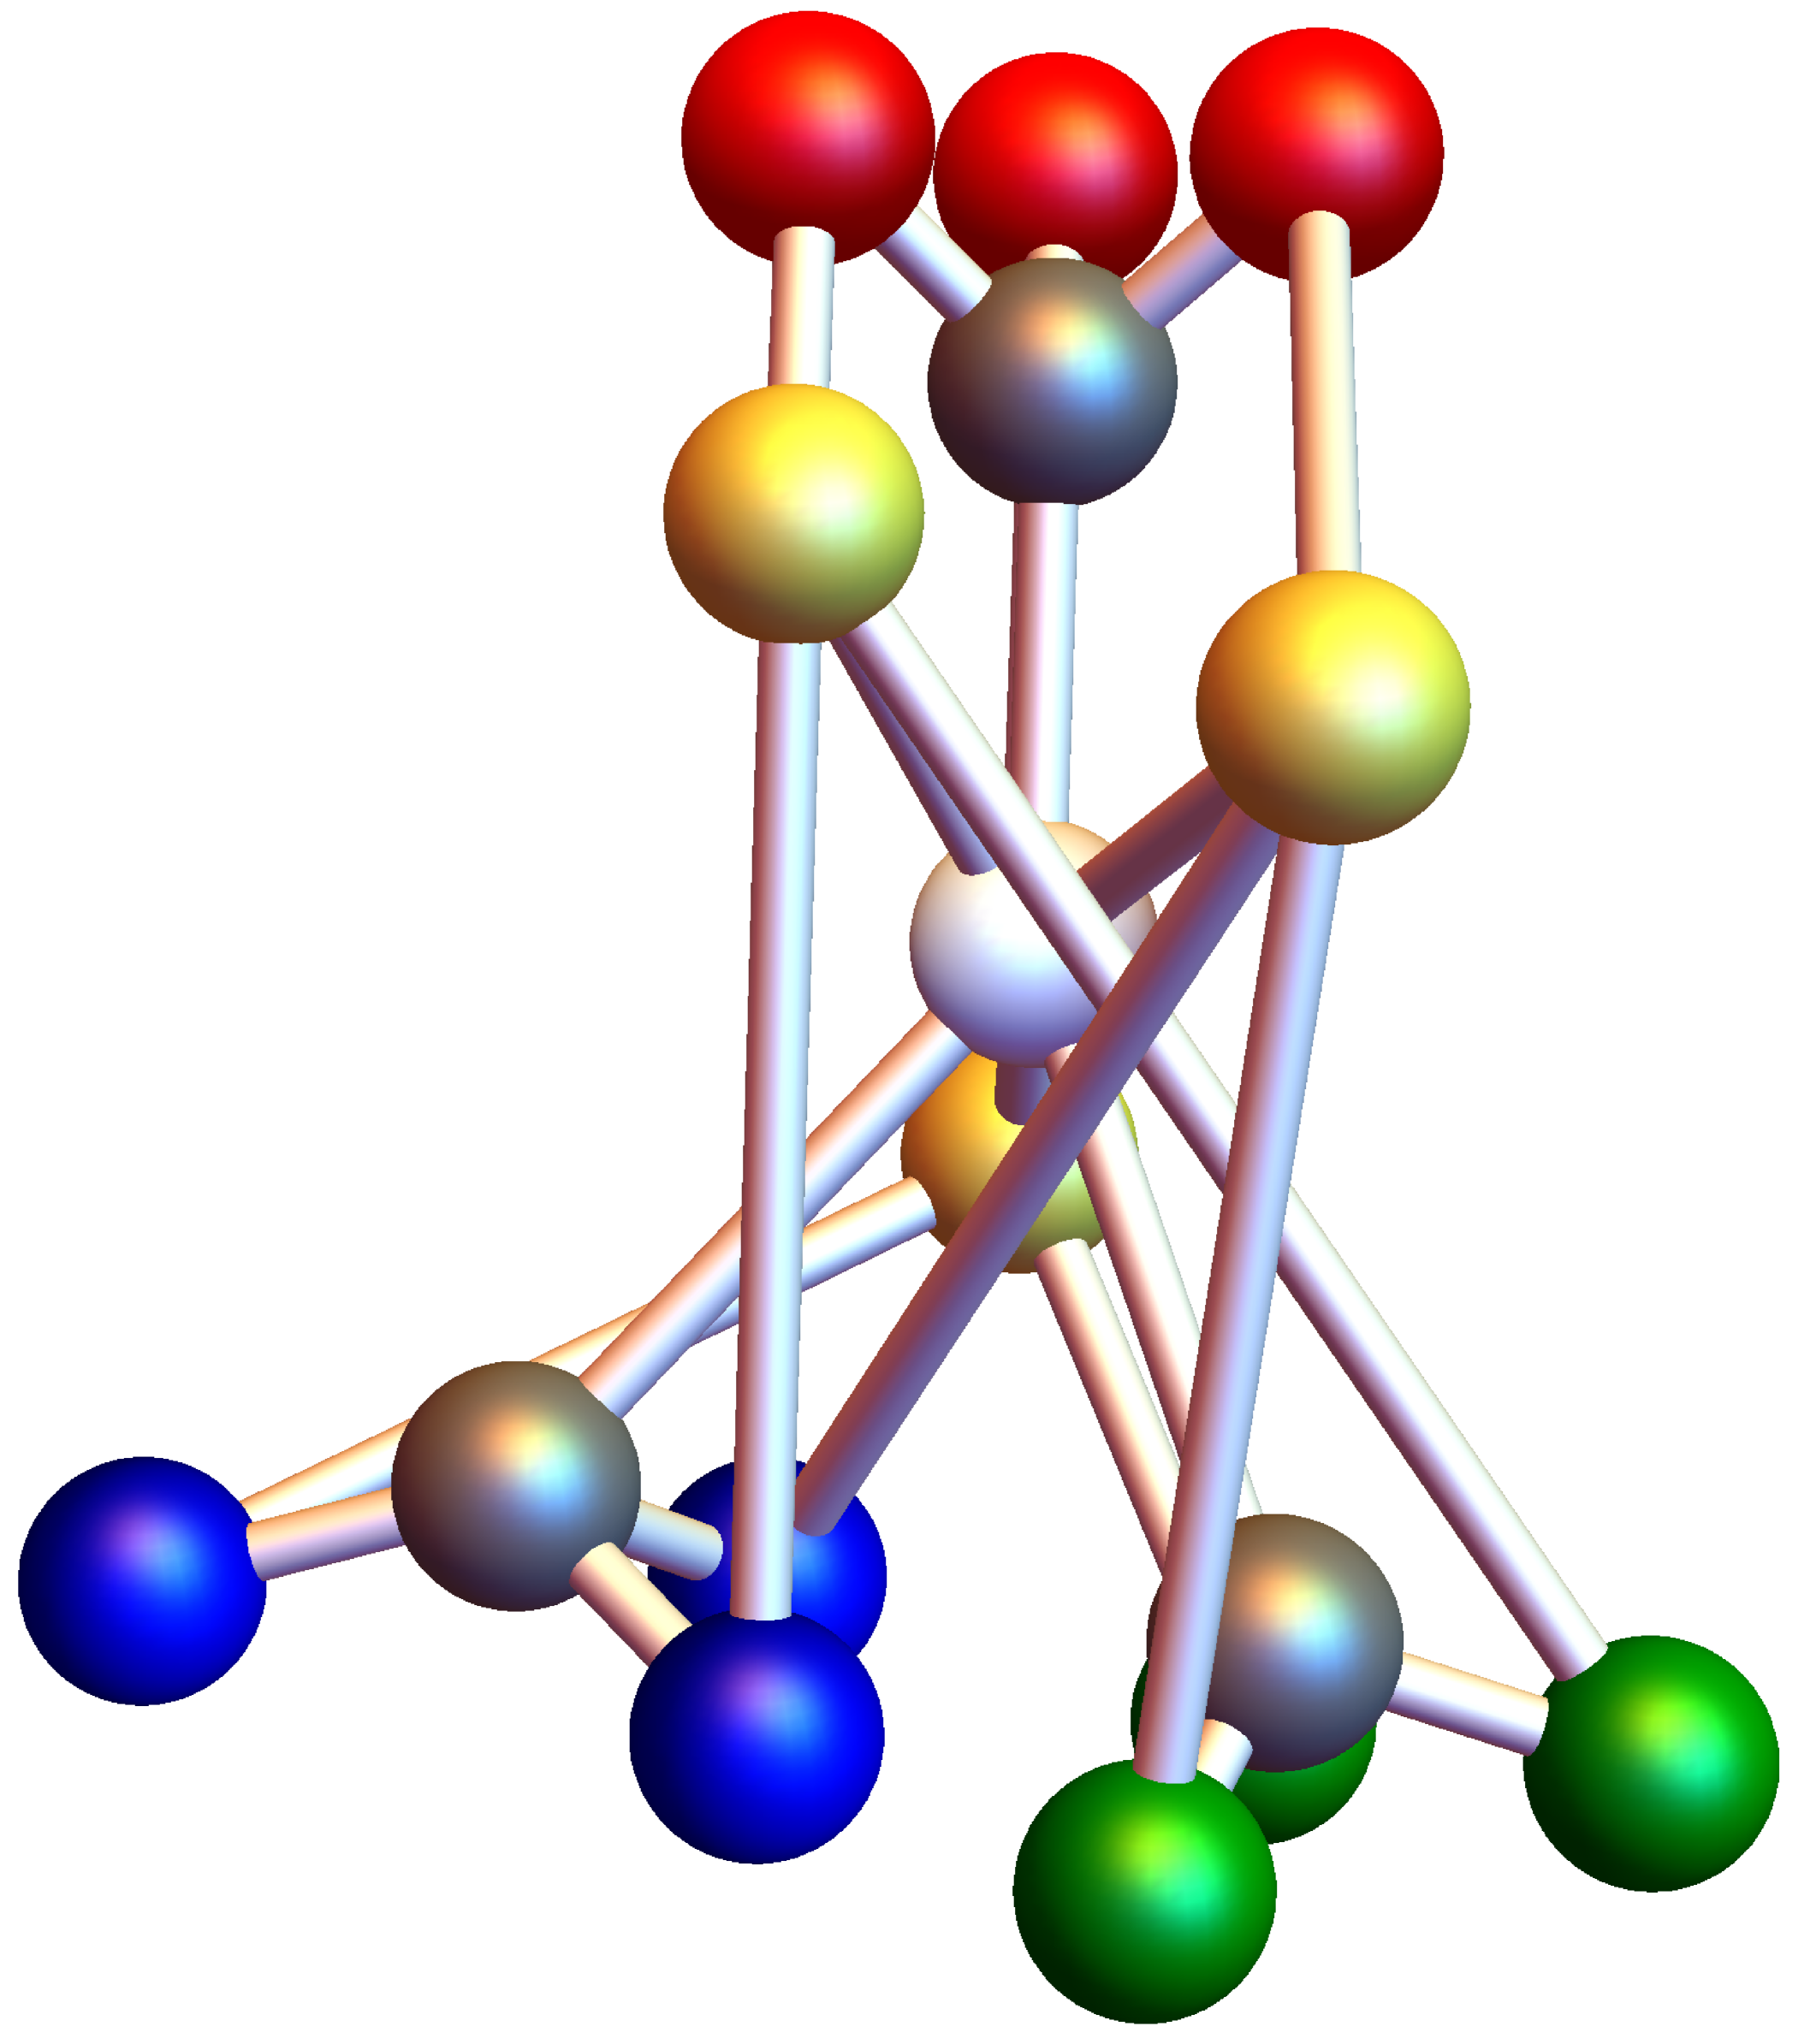
\includegraphics[width=0.3\textwidth]{Images/switch_square}\\[1cm]
	\vfill
\end{titlepage}

\tableofcontents}


\section{Classical Computation}

\subsection{Of Bits and Bytes}
\mode<presentation>{\begin{frame}{Of Bits and Bytes}\label{register}
			\centering\vspace*{1.0cm}
   	\begin{itemize}
   		\item Computers operate on \textsc{registers}
   		\item Composed of $n$ switches $\rightarrow$ \textsc{bits}
   		\item Two discrete states per switch, \textsc{on} and \textsc{off}
   		\item Represents numbers between $0$ and $2^n - 1$
   	\end{itemize}
   	\vspace{1.2cm}
    \includegraphics[trim=0 0 0 0mm, width=0.7\textwidth]{Images/bitregister}
\end{frame}}

\begin{center}
	\includeslide{register}
\end{center}

\noindent text 

\subsection{Turing Machine}
\mode<presentation>{\begin{frame}{Turing Machine}\label{turing}
	\begin{columns}[T]
		\begin{column}{0.4\textwidth}
			\centering\vspace*{0.5cm}
   			\begin{itemize}
   				\item Read/write head and register
   				\item Reads one \textsc{bit}
   				\item Manipulates \textsc{bit} according to program
   			\end{itemize}
		\end{column}
		\begin{column}{0.6\textwidth}
			\centering
    		\includegraphics[trim=0 0 0 0mm, width=\textwidth]{Images/turingMachine}
		\end{column}
	\end{columns}
\end{frame}}

\begin{center}
	\includeslide{turing}
\end{center}

\noindent text

\subsection{Computational Complexity}
\mode<presentation>{\begin{frame}{Computational Complexity}\label{complexity}
%	\begin{columns}[T]
%		\begin{column}{0.5\textwidth}
%			\centering\vspace*{0.0cm}
%   			\begin{itemize}
%   				\item Resource demand depending on input size
%   				\item Asymptotic behavior
%   				\item Roughly: exponential complexity means inefficient algorithm
%   				\item Foundation for public key cryptography
%   			\end{itemize}
%		\end{column}
%		\begin{column}{0.5\textwidth}
			\centering
			\Large
    		\begin{table}
				\begin{tabular}{l | c }
					Task & Complexity \\
					\hline \hline
					Multiplication & $\mathcal{O}(n\log(n)2^{\mathcal{O}(\log^*(n))})$ \\
					Factorial & $\mathcal{O}(M(n \log(n)))$ \\
					MatMult & $\mathcal{O}(n^{2.737})$ \\
					Factorization & $\mathcal{O}(\exp(\sqrt[3]{\frac{64}{9}}n\log^2(n)))$ \\
					List search & $\mathcal{O}(n)$ 
				\end{tabular}
			%\caption{Complexity}
			\end{table}
			\normalsize
%		\end{column}
%	\end{columns}
	\vspace*{1.0cm}
	Linear input growth $\rightarrow$ Exponential system demand\\
	Bad!
\end{frame}}

\begin{center}
	\includeslide{complexity}
\end{center}

\noindent text

\section{Quantum Computation}
\subsection{Qubits}
\mode<presentation>{\begin{frame}{Qubits}\label{qubits}
	\begin{itemize}
		\item $2$ distinguishable states $\ket{0}$ and $\ket{1}$
		%\item Usually spin-$\frac{1}{2}$ systems ($\ket{\uparrow}$ and $\ket{\downarrow}$)
		\item $\ket{0}$ and $\ket{1}$ are basis vectors of the associated \\\textsc{Hilbert space} $\mathbb{H}_2$
		\item General state
			\begin{align*}
				\ket{\Psi} &= \alpha\ket{0} + \beta\ket{1} \\
				\bra{\Psi} &= \alpha^*\bra{0} + \beta^*\bra{1}
			\end{align*}
		\text{with} $\quad \alpha, \beta \in \mathbb{C}$
		\item Independent: $\braket{0|1} = 0$
		\item Normalized: $\braket{0|0} = 1$, $\braket{1|1} = 1$
	\end{itemize}
\end{frame}}

\begin{center}
	\includeslide{qubits}
\end{center}

\noindent text

\mode<presentation>{\begin{frame}{Measurement}\label{measurement}
	\begin{columns}[T]
		\begin{column}{0.5\textwidth}
			\centering\vspace*{0.3cm}
   			\begin{itemize}
   				\item Probability to find $\ket{0}$
   					\[\text{p}(\ket{0}) = \ket{0}\braket{0|\Psi} = |\alpha|^2\]
   				\item Probability to find $\ket{0}$ or $\ket{1}$
   					\[\text{p}(\ket{0})+\text{p}(\ket{1}) = |\alpha|^2 + |\beta|^2 = 1\]
   				\item States are normalized 
   					\[\ket{\Psi} = \cos{\left(\frac{\Theta}{2}\right)} \ket{0} + e^{\text{i}\phi}\sin{\left(\frac{\Theta}{2}\right)}\ket{1}\]
   			\end{itemize}
		\end{column}
		\begin{column}{0.5\textwidth}
			\centering
    		\includegraphics[trim=-5mm 0 0 0mm, width=0.9\textwidth]{Images/bloch_sphere}
		\end{column}
	\end{columns}
\end{frame}}

\begin{center}
	\includeslide{PST}
\end{center}

\noindent text


\mode<presentation>{\begin{frame}[t]{Quantum Register}\label{qregister}
	\begin{itemize}
		\item Classical: cartesian product of state spaces
			\[S^\text{full} = S_1 \times S_2 \times \dots \times S_N\] 
		\[\text{dim}(S^\text{full}) = N\cdot f\]
		\item Quantum: tensor product of Hilbert spaces
			\[\mathbb{H}^{\text{full}} = \mathbb{H}_1 \otimes \mathbb{H}_2 \otimes \dots \otimes \mathbb{H}_N\] 
	\end{itemize}
	\begin{exampleblock}{}
		\setlength\abovedisplayskip{-8pt}
		\begin{center}
			$\text{dim}(\mathbb{H}^{full}) = f^N$
		\end{center}
	\end{exampleblock}
\end{frame}}


\mode<presentation>{\begin{frame}[t]{Quantum Register}\label{qregister2}
	\begin{itemize}
		\vspace*{1.5cm}
		\item Basis vectors: 
			\[\ket{0}\otimes\ket{0}, \ket{0}\otimes\ket{1}, \ket{1}\otimes\ket{0}, \ket{1}\otimes\ket{1}\]
		\item Short: 
			\[\ket{00}, \ket{01}, \ket{10}, \ket{11}\]
		\item System $2$ in superposition $\ket{\Psi_2} = \alpha\ket{0} + \beta\ket{1}$, register state
			\[\ket{\Psi} = \alpha\ket{0000} + \beta\ket{0100}\]
	\end{itemize}
\end{frame}}

\begin{center}
	\includeslide{qregister}
\end{center}

\noindent text

%\mode<presentation>{\begin{frame}[t]{Entanglement}\label{entanglement}
%	\begin{itemize}
%		\item Unentangled states can be decomposed
%			\[\ket{\Psi_u} = \frac{1}{\sqrt{2}}(\ket{00} + \ket{01}) = \ket{0} \otimes \frac{1}{\sqrt{2}}(\ket{0} + \ket{1})\]
%		\item Entangled states states cannot
%			\[\ket{\Psi_e} = \frac{1}{\sqrt{2}}(\ket{00} + \ket{11}) \]
%		\item zio
%	\end{itemize}
%\end{frame}}
%
%\begin{center}
%	\includeslide{entanglement}
%\end{center}
%
%\noindent text


\mode<presentation>{\begin{frame}[t]{Quantum Parallelism}\label{quantumparallel}
	\begin{itemize}
		\item Step 1: Partition the register
			\[\ket{00000} \rightarrow \ket{0000;0} \]
		\item Step 2: Full input Superposition 
			\[\ket{\Psi} = \frac{1}{\sqrt{N}}(\ket{0000;0} + \ket{0001;0} + \dots + \ket{1111;0}) = \frac{1}{\sqrt{N}}\sum^{2^N-1}_{a=0}\ket{a;0}\]
		\item Step 3: Apply quantum gates
			\[U_f\ket{\hat{\Psi}} = \sum^{2^N-1}_{a=0}\ket{a;f(a)} = \frac{1}{\sqrt{N}}(\ket{0000;f(0000)} + \ket{0001;f(0001)} + \dots)\]
		%\item Step 4: Extract result
	\end{itemize}
	%$\rightarrow$ Result is calculated on all input states at once!
\end{frame}}

\begin{center}
	\includeslide{quantum parallel}
\end{center}

\noindent text

\subsection{Result Extraction}

\mode<presentation>{\begin{frame}{Quantum Fourier Transformation}\label{qft}
		\begin{center}
			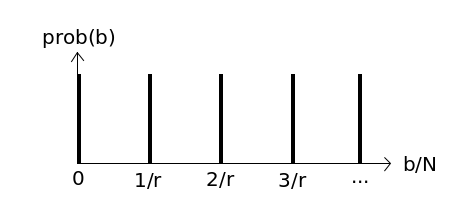
\includegraphics[trim=0 0 0 0mm, width=0.8\textwidth]{Images/qftperiod}
			\[\ket{\tilde{\Psi}} = \frac{1}{N}\sum_{a=0}^{2^N-1}\sum_{b=0}^{2^N-1}\text{e}^{2\pi i a b/N}\ket{b;f(a)}\]
		\end{center}
			\begin{itemize}
				\item Measure random multiple of $1/r$
				\item Repeat $\mathcal{O}(\log\log{\frac{r}{N}})$ times 
				\item Shor's algorithm: find period of 
					\[f(x) = a^x\,\, \text{mod}\,\, N\]
			\end{itemize}
\end{frame}}

\begin{center}
	\includeslide{qft}
\end{center}

\noindent Fermat's little theorem


\mode<presentation>{\begin{frame}[t]{Amplitude Amplification}\label{amplification}
	\begin{center}
		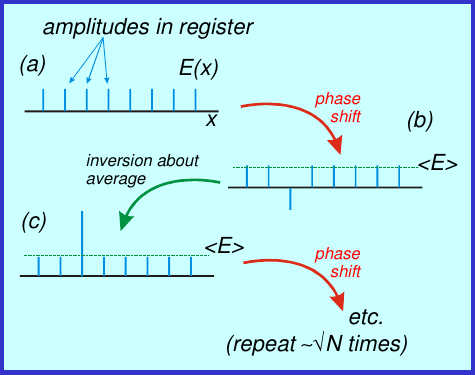
\includegraphics[trim=0 0 0 0mm, width=0.8\textwidth]{Images/amplitudeamplification} \\
	\end{center}	
	\footnotesize\textcolor{tugreen}{$\blacktriangleright$}\,\,\cite{Spreeuw}\normalsize
	
\end{frame}}

\begin{center}
	\includeslide{amplification}
\end{center}

\noindent text



\mode<presentation>{\begin{frame}{Quantum Random Walk}\label{qrw}
	\begin{columns}[T]
		\begin{column}{0.5\textwidth}
			\centering
			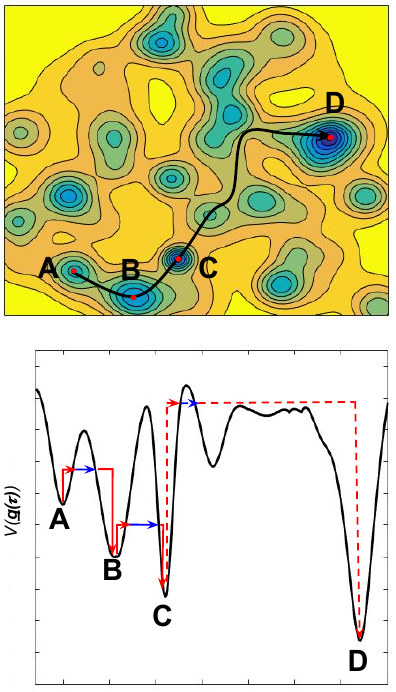
\includegraphics[trim=0 0 0 0mm, width=0.75\textwidth]{Images/quantumrandomwalk}
		\end{column}
		\begin{column}{0.5\textwidth}
			\centering
    		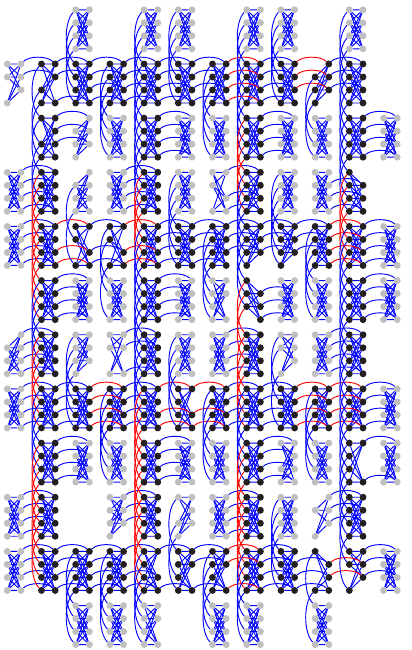
\includegraphics[trim=0 0 0 0mm, width=0.8\textwidth]{Images/exampled-wave}
		\end{column}
	\end{columns}
	\footnotesize\textcolor{tugreen}{$\blacktriangleright$}\,\,\cite{Denchev2015}\normalsize
\end{frame}}

\begin{center}
	\includeslide{qrw}
\end{center}

\noindent text

\mode<presentation>{\begin{frame}[t]{QC Strengths}\label{strengths}
	\centering
	\Large
	\begin{table}
		\begin{tabular}{l | c }
			Task & Complexity \\
			\hline \hline
			Discrete log & $\mathcal{O}(n^3)$ \\
			Verify MatMult & $\mathcal{O}(n^\frac{5}{3})$ \\
			$k$ Fake Coins & $\mathcal{O}(k^\frac{1}{4})$ \\
			Factorization & $\mathcal{O}(n^3)$ \\
			List search & $\mathcal{O}(\sqrt{n})$ 
		\end{tabular}
	%\caption{Complexity}
	\end{table}
	\normalsize
	\begin{itemize}
		\item Optimization
		\item Big Data
		\item Artificial Intelligence
	\end{itemize}
	\vspace*{0.5cm}
	See \textsc{NIST} Quantum Algorithm Zoo for more
\end{frame}}


\begin{center}
	\includeslide{strengths}
\end{center}

\noindent text

\mode<presentation>{\begin{frame}[t]{D-Wave 2000Q}\label{dwave}
	\begin{columns}[T]
		\begin{column}{0.5\textwidth}
			\centering
			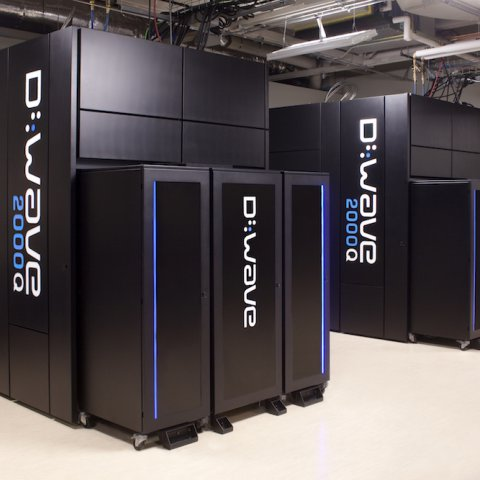
\includegraphics[trim=0 0 0 0mm, width=0.75\textwidth]{Images/d-wave2000q.jpg} \\
			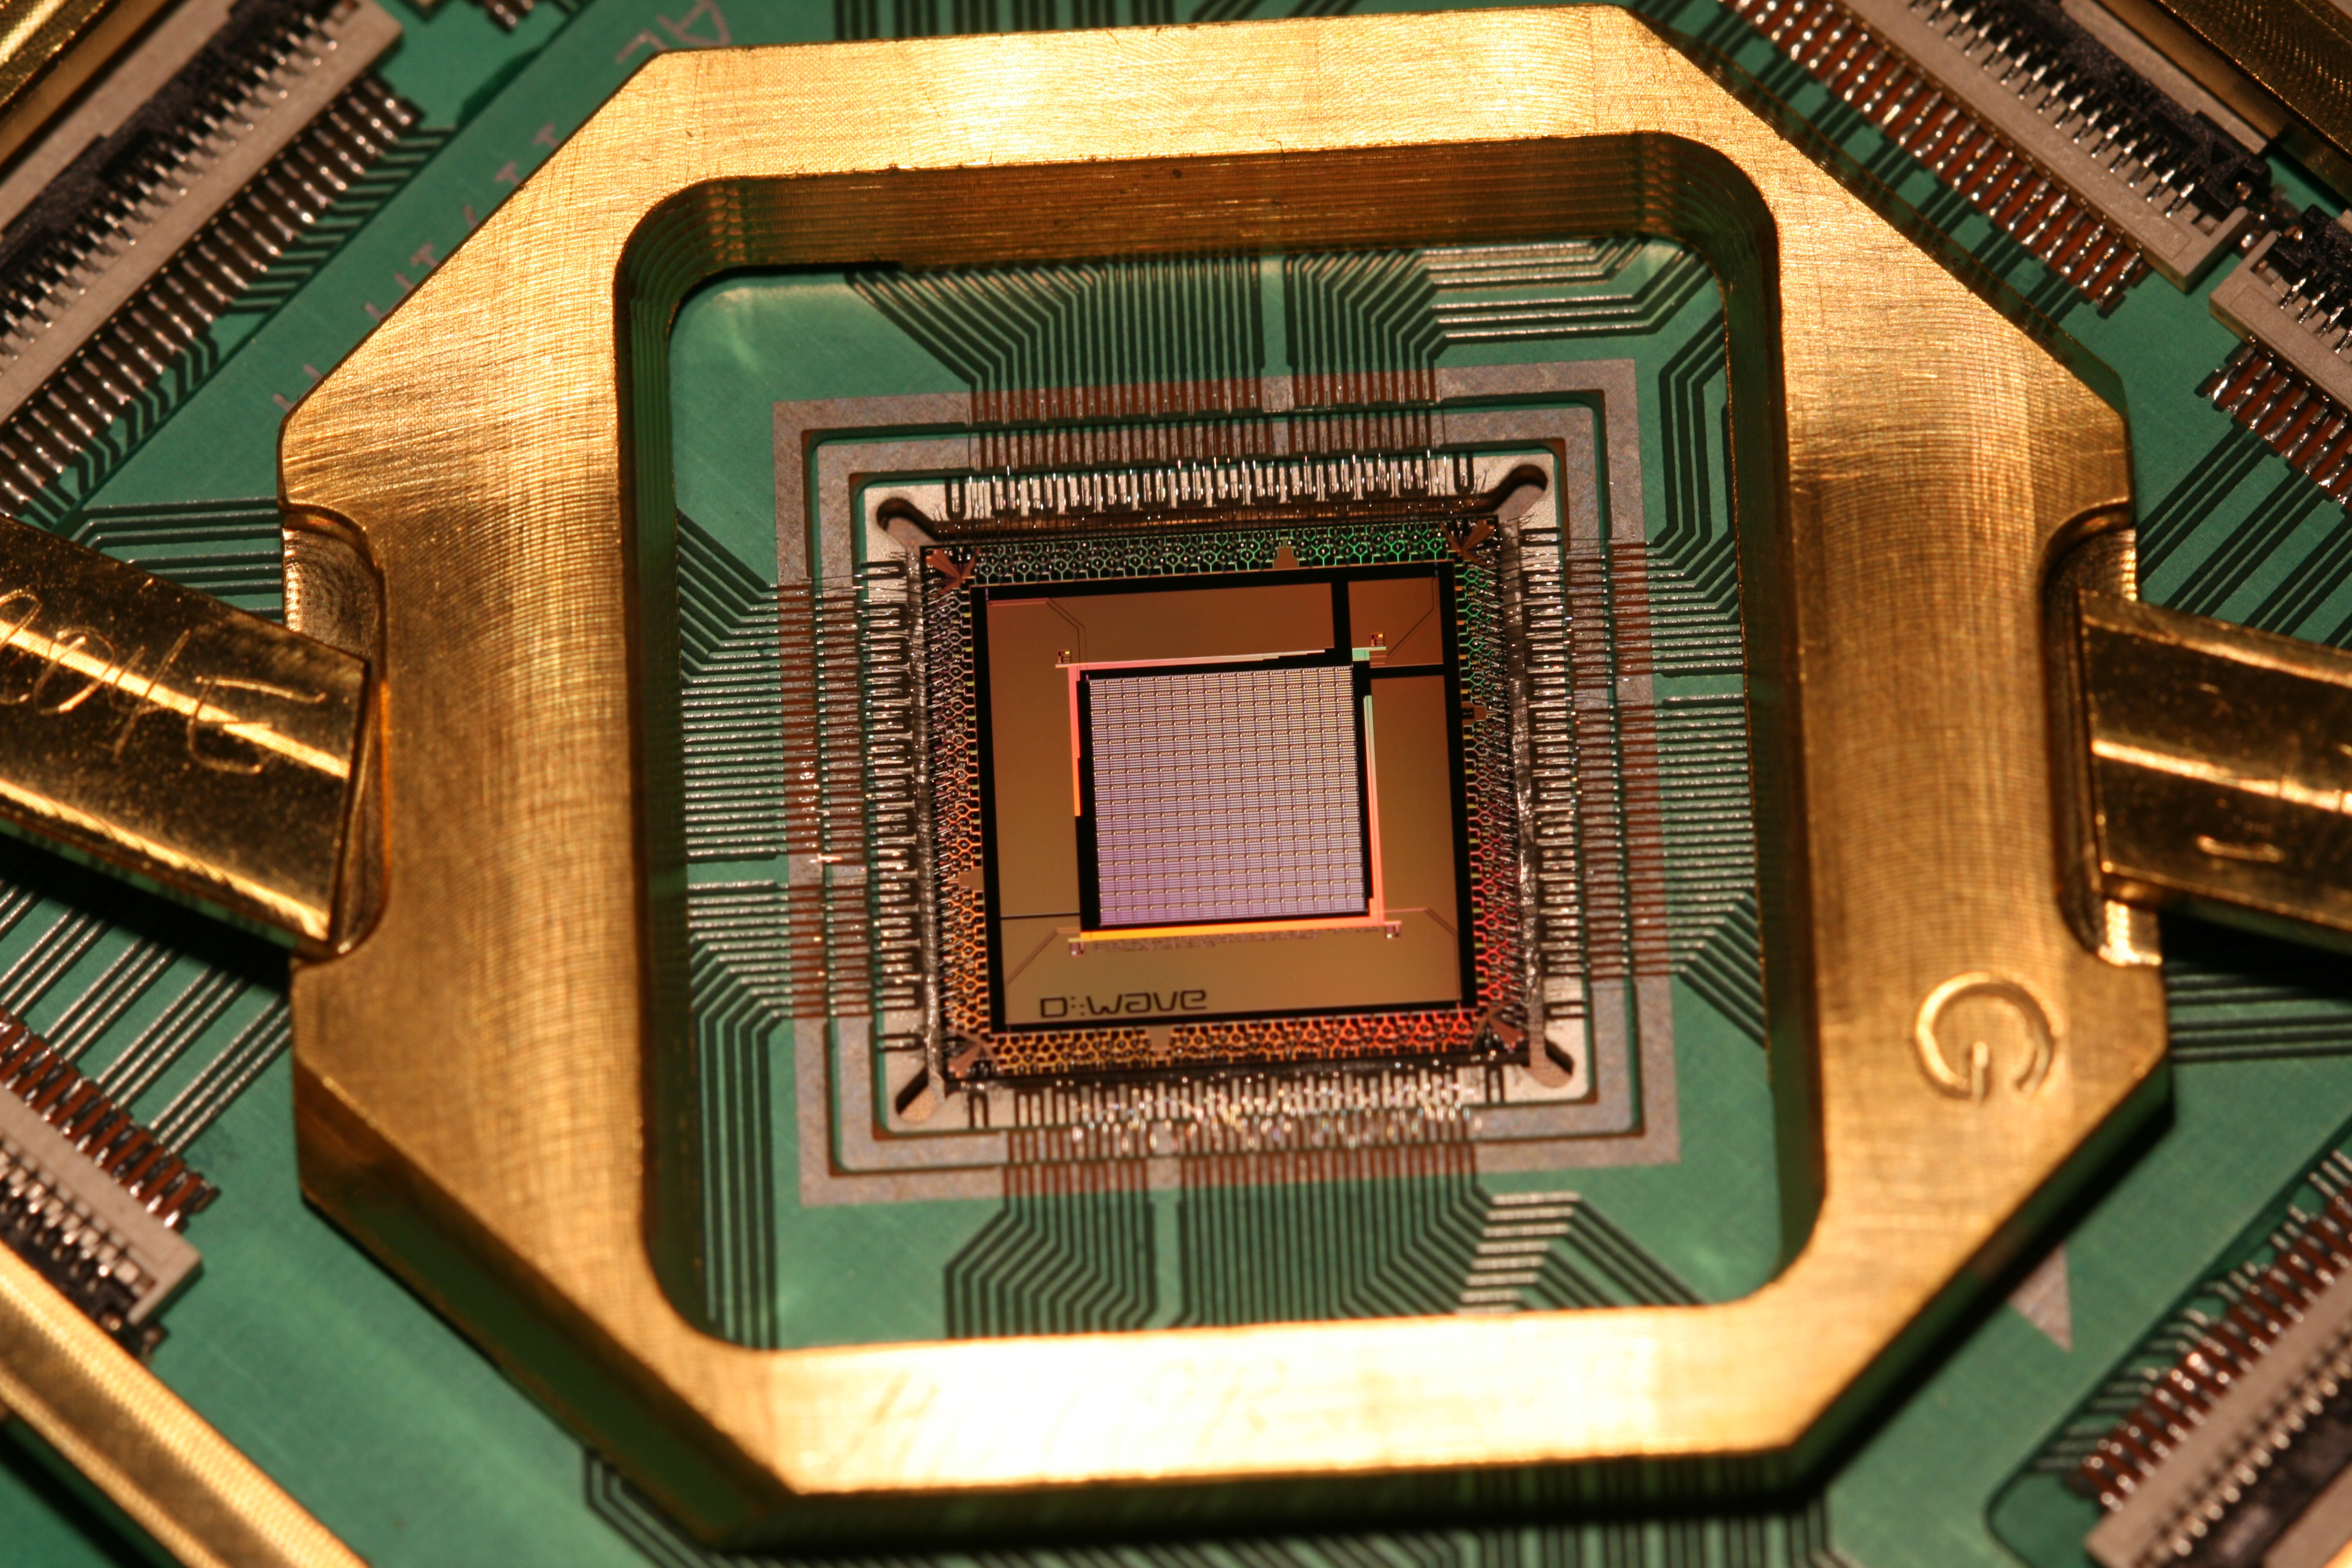
\includegraphics[trim=0 0 0 0mm, width=0.75\textwidth]{Images/d-wave-processor.jpg}
		\end{column}
		\begin{column}{0.5\textwidth}
			\centering
			\begin{itemize}
				\item Quantum Annealer
				\item $2000$ squids 
				\item $25$\,kW vs. $\mathcal{O}(1000)$\,kW
				\item Temperature $0.015$\,K
			\end{itemize}
			\vspace*{0.5cm}
    		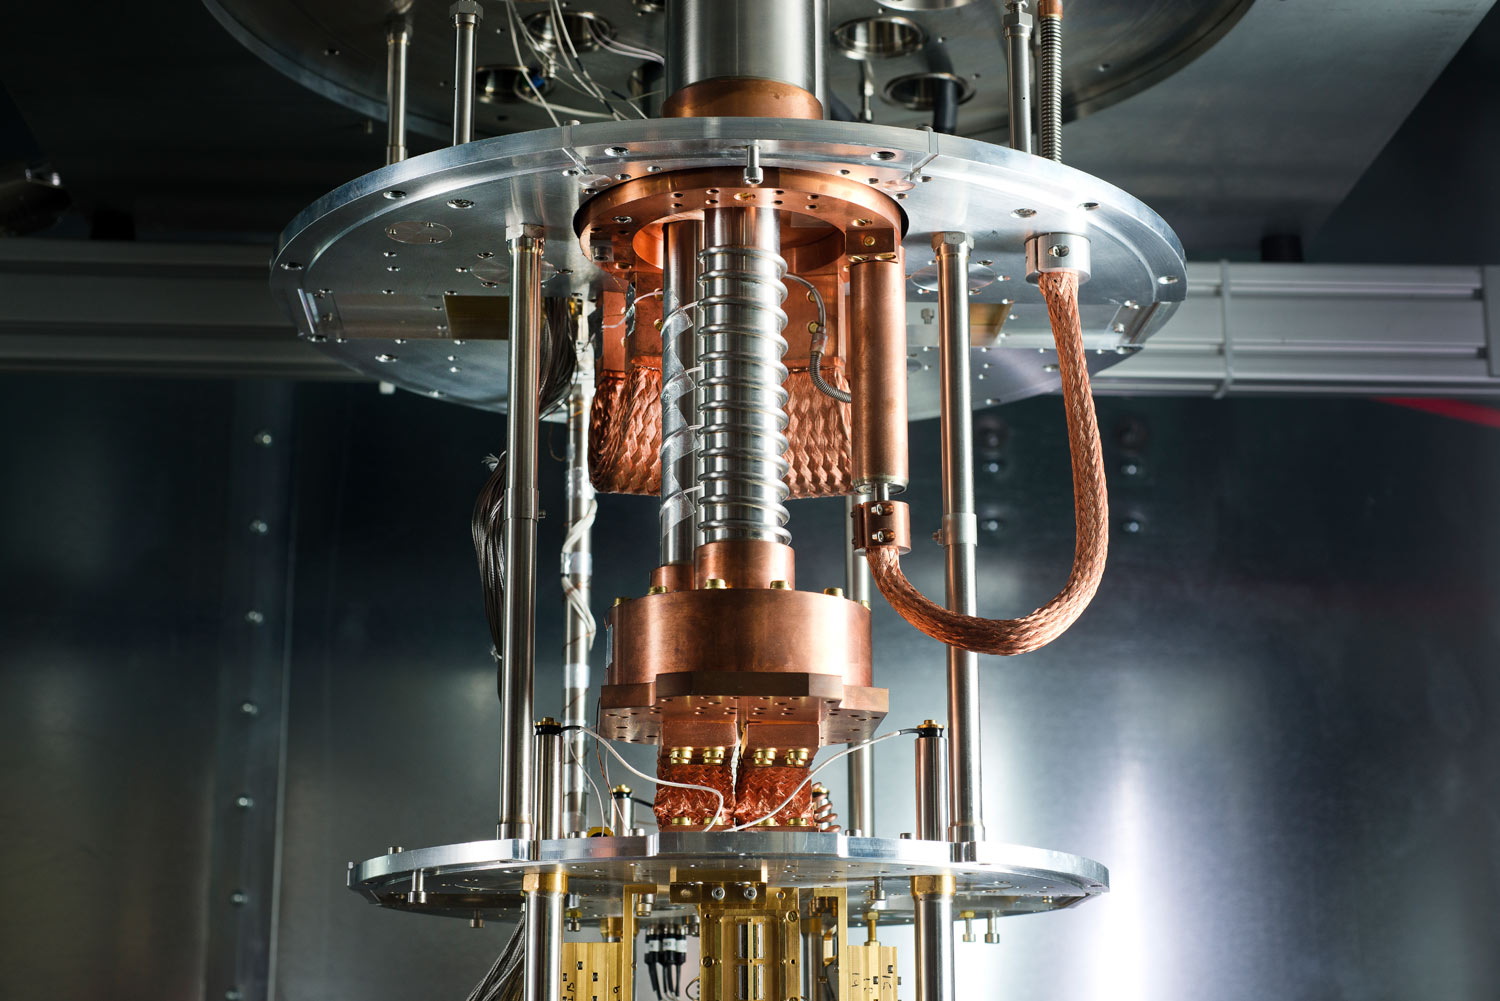
\includegraphics[trim=0 0 0 0mm, width=0.9\textwidth]{Images/cryostate.jpg}
		\end{column}
	\end{columns}
	\vspace*{0.5cm}
	\footnotesize\textcolor{tugreen}{$\blacktriangleright$}\,\,\cite{Inc.2016}\normalsize
\end{frame}}


\begin{center}
	\includeslide{dwave}
\end{center}

\noindent text


\mode<presentation>{\begin{frame}{Universal QC}\label{uniqc}
	\begin{columns}[T]
		\begin{column}{0.5\textwidth}
			\centering
			NMR \\
			\vspace{0.3cm}
			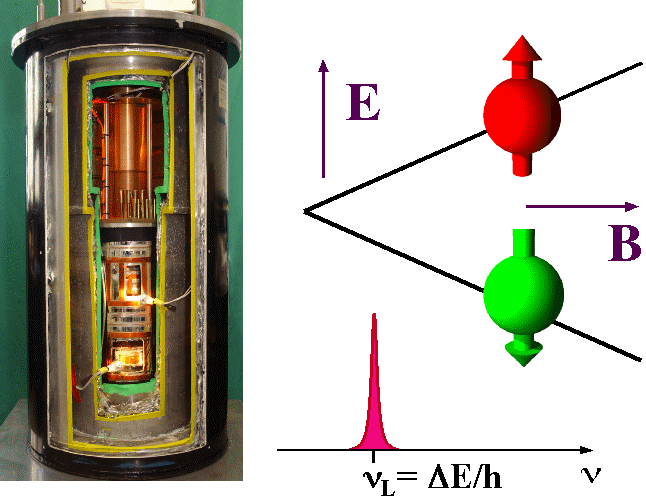
\includegraphics[trim=0 0 0 0mm, width=0.75\textwidth]{Images/nmr-e3} \\
			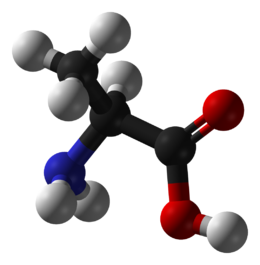
\includegraphics[trim=0 0 0 0mm, width=0.6\textwidth]{Images/nmr-alanine}
		\end{column}
		\begin{column}{0.5\textwidth}
			\centering
			Transmons \\
			\vspace{0.3cm}
    		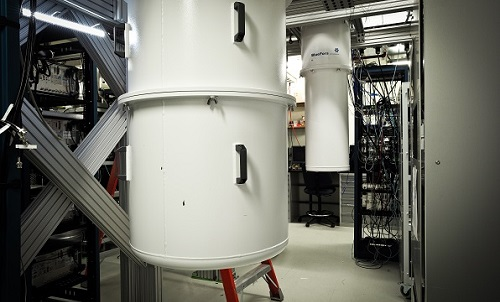
\includegraphics[trim=0 0 0 0mm, width=0.9\textwidth]{Images/ibm-cryo.jpg} \\
    		\vspace*{1.0cm}
    		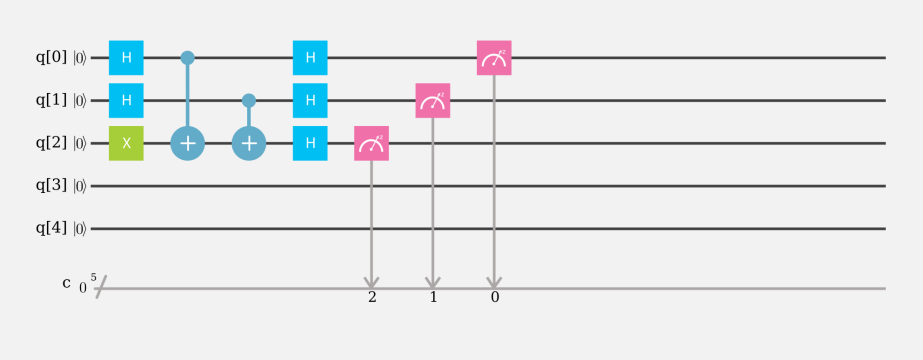
\includegraphics[trim=0 0 0 0mm, width=0.95\textwidth]{Images/ibm-composer} \\
    		Cloud-accessible!
		\end{column}
	\end{columns}
	\vspace*{0.3cm}
	\footnotesize\textcolor{tugreen}{$\blacktriangleright$}\,\,\cite{Computing2017}\normalsize
\end{frame}}

\begin{center}
	\includeslide{uniqc}
\end{center}

\noindent text

\section{Spin Networks}

\mode<presentation>{\begin{frame}[t]{QC Architecture}\label{architecture}
	\begin{columns}[T]
		\begin{column}{0.5\textwidth}
			\centering
   			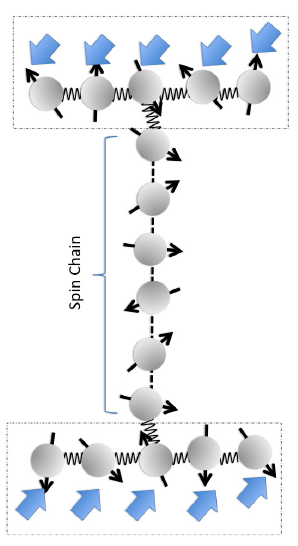
\includegraphics[trim=0mm 0 0 0mm, width=0.7\textwidth]{Images/processor}
		\end{column}
		\begin{column}{0.5\textwidth}
			\vspace*{1.0cm}
			\begin{itemize}
    			\item Distributed components
    			\item Smaller system size $\rightarrow$ less disturbance
    			\item Quantum wires without external control
    			\item Same material as processor
    		\end{itemize}
    		\vspace*{1.0cm}
    		$\rightarrow$ Spin Networks
		\end{column}
	\end{columns}
   	\footnotesize\textcolor{tugreen}{$\blacktriangleright$}\,\,\cite{Bose2014}\normalsize
\end{frame}}


\begin{center}
	\includeslide{architecture}
\end{center}

\noindent text


\mode<presentation>{\begin{frame}{Perfect State Transfer}\label{pst} %[fragile,t] for listings
	\begin{exampleblock}{}
	\setlength\abovedisplayskip{-8pt}
	\begin{center}
		\[H_{XX}=\frac{1}{2}J\sum_{i=1}^{N}{\left[\sigma_i^x\sigma_{i-1}^x + \sigma_i^y\sigma_{i-1}^y\right]}\]
	\end{center}
	\end{exampleblock} 
	Perfect State Transfer happens if
	\[ \mathfrak{F}(t) = \frac{\lvert f^N_{r,s}(t)\rvert\cos{\lambda}}{3} + \frac{\lvert f^N_{r,s}(t)\rvert^2}{6} + \frac{1}{2} = 1\]
	\vspace*{-0.7cm}
	\begin{exampleblock}{}
	\setlength\abovedisplayskip{-8pt}
	\begin{center}
		\[\lvert f^N_{r,s}(t)\rvert = \lvert \braket{r|\text{e}^{-iHt}|s}\rvert = 1\]
	\end{center}
	\end{exampleblock}
\end{frame}}

\begin{center}
	\includeslide{pst}
\end{center}

\noindent text


\mode<presentation>{\begin{frame}{Graphs}\label{graphs}
	\begin{exampleblock}{}
	\setlength\abovedisplayskip{-8pt}
	\begin{center}
		$G = (V,E)$
	\end{center}
	\end{exampleblock}
	Example: $V = \{1,2,3\}, E = \{\{1,2\},\{2,3\}\}$
	\begin{center}
		\includegraphics[trim=0mm 0 0 0mm, width=0.7\textwidth]{Images/chain3-graph}
	\end{center}
	Algebraic treatment through adjacency matrices:
	\begin{exampleblock}{}
	\setlength\abovedisplayskip{-8pt}
	\begin{center}
		$a_{ij} = \left\{
	\begin{array}{ll}
		1  & \{i,j\} \in E \\
		0  & \text{otherwise}
	\end{array}
\right.$	
	\end{center}
	\end{exampleblock}
\end{frame}}

\begin{center}
	\includeslide{graphs}
\end{center}

\noindent text


\mode<presentation>{\begin{frame}{Examples}\label{adjexamples}
	\begin{columns}[T]
		\begin{column}{0.5\textwidth}
			\centering
			\vspace{1.5cm}
   			\includegraphics[trim=0mm 0 0 0mm, width=0.7\textwidth]{Images/chain3} \\
   			\vspace{1.0cm}
   			\includegraphics[trim=0mm 0 0 0mm, width=0.7\textwidth]{Images/chain3-adjmat}
		\end{column}
		\begin{column}{0.5\textwidth}
			\centering
   			\includegraphics[trim=0mm 0 0 0mm, width=0.6\textwidth]{Images/chain6vary-graph} \\
   			\includegraphics[trim=0mm 0 0 0mm, width=0.7\textwidth]{Images/chain6vary-adjmat}
		\end{column}
	\end{columns}
\end{frame}}

\begin{center}
	\includeslide{adjexamples}
\end{center}

\noindent text


\mode<presentation>{\begin{frame}{Identifying PST Graphs}\label{identifyPST}
	\begin{center}
		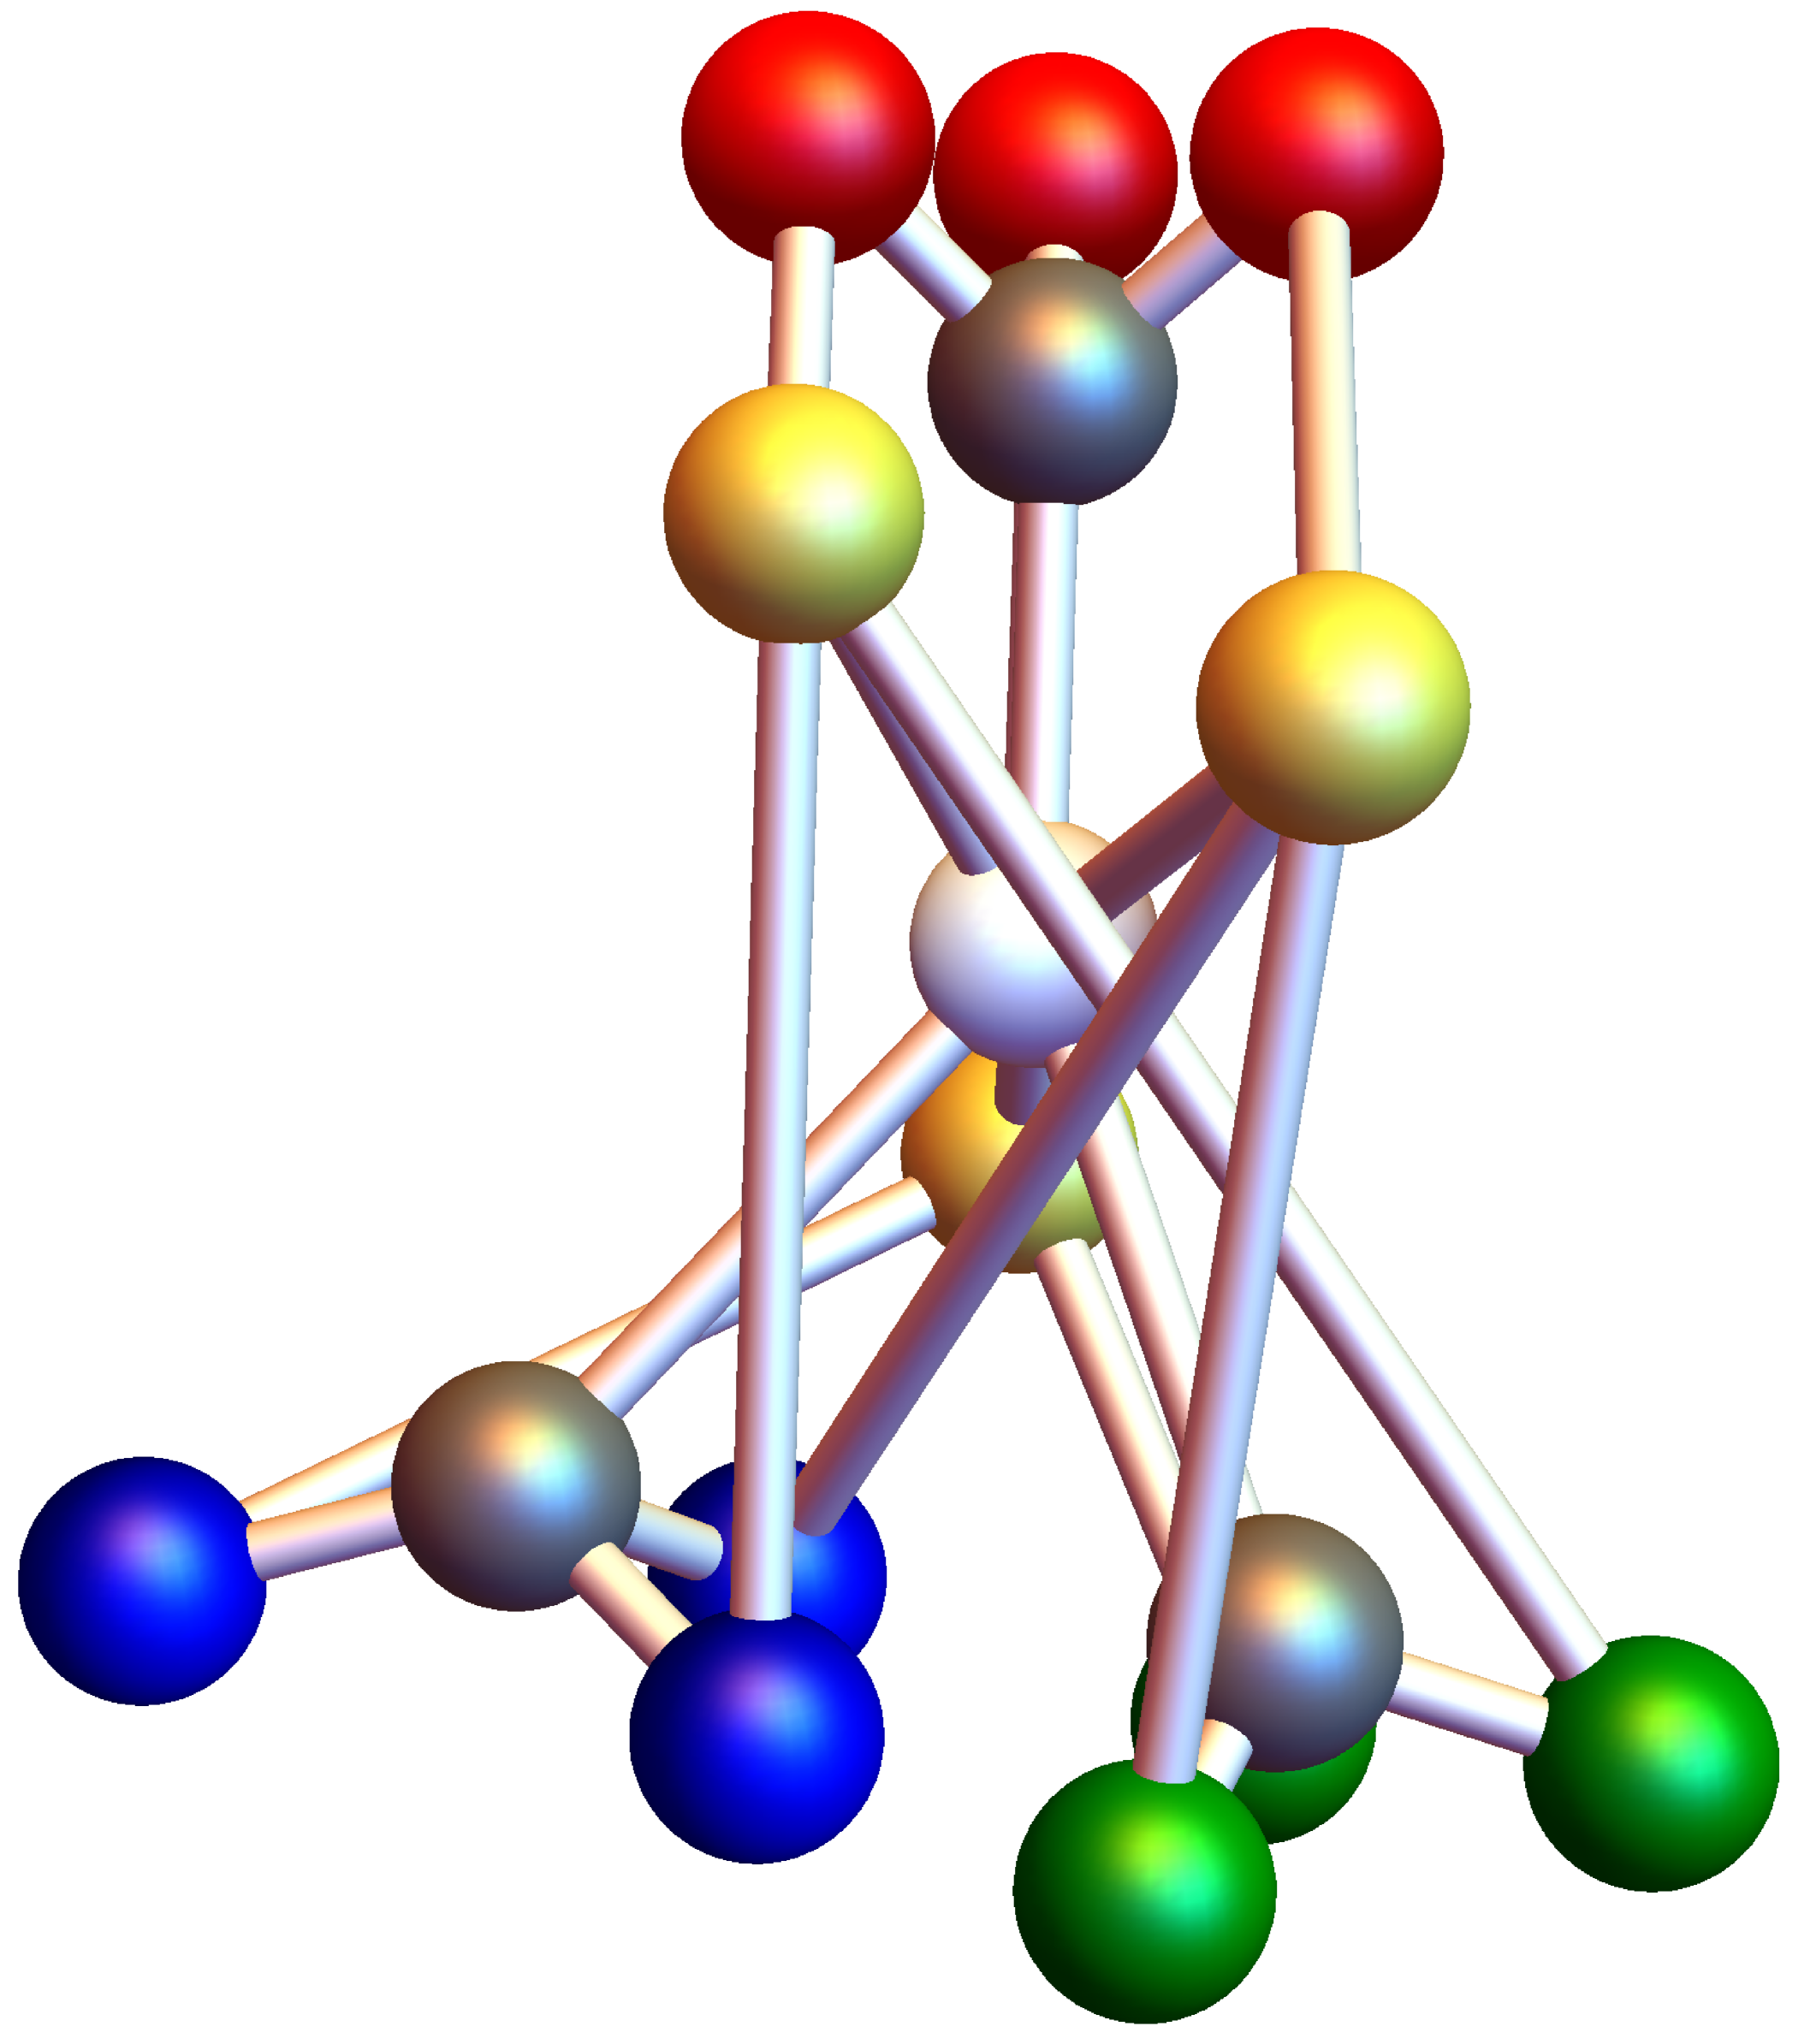
\includegraphics[trim=0mm 0 0 0mm, width=0.5\textwidth]{Images/switch_square}
	\end{center}
	\begin{itemize}
		\item Transport part of an entangled pair along the network
		\item Entangle separated parts of a system
		\item Quantum teleportation as transportation scheme
	\end{itemize}
\end{frame}}

\begin{center}
	\includeslide{identifyPST}
\end{center}

\noindent text


\mode<presentation>{\begin{frame}{Graph Product}\label{graphproduct}
	\begin{exampleblock}{}
	\setlength\abovedisplayskip{-8pt}
	\begin{center}
		$A_{G\times H} = A_G \otimes \mathfrak{1}_{\left|V_H\right|} + \mathfrak{1}_{\left|V_G\right|} \otimes A_H$
	\end{center}
	\end{exampleblock}
	\begin{columns}[T]
		\begin{column}{0.33\textwidth}
			\centering
   			\includegraphics[trim=0mm 0 0 0mm, width=1.0\textwidth]{Images/graphprod_chain3_square} \\
		\end{column}
		\begin{column}{0.33\textwidth}
			\centering
   			\includegraphics[trim=0mm 0 0 0mm, width=1.0\textwidth]{Images/graphprod_chain3_chain2_square} \\
		\end{column}
		\begin{column}{0.33\textwidth}
			\centering
   			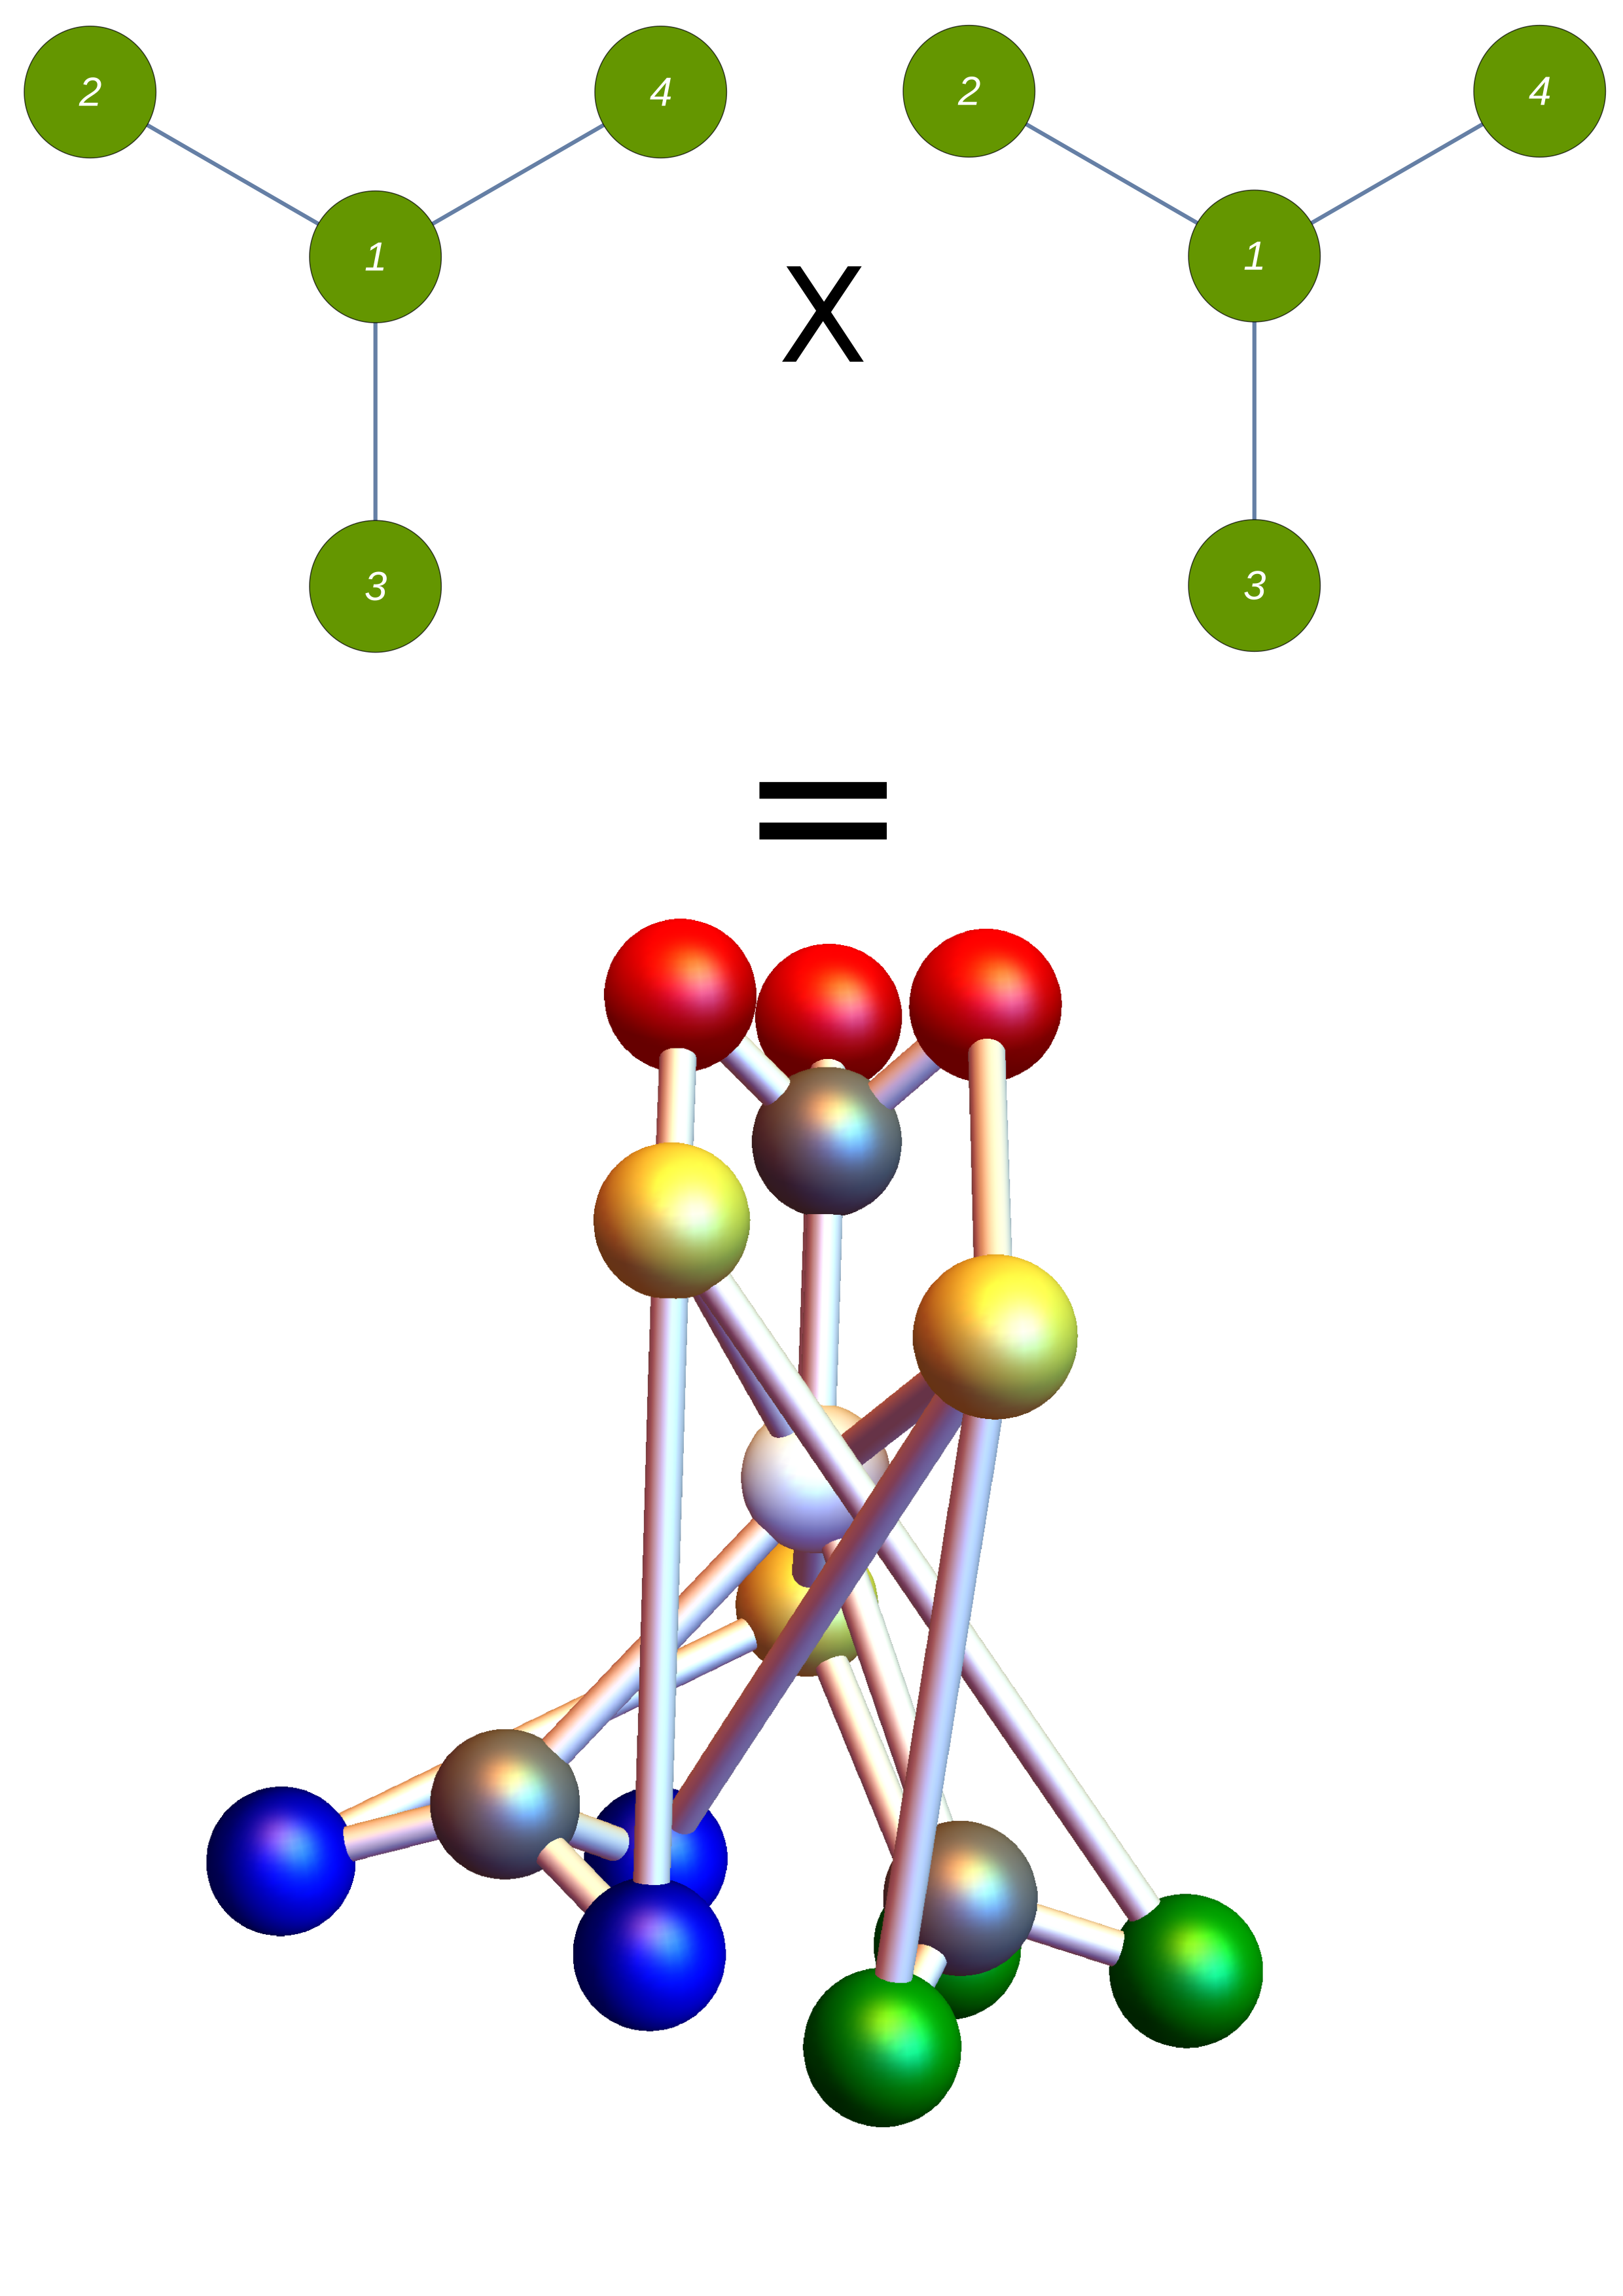
\includegraphics[trim=0mm 0 0 0mm, width=1.0\textwidth]{Images/graphprod_switch_square.pdf} \\
		\end{column}
	\end{columns}
\end{frame}}

\begin{center}
	\includeslide{graphproduct}
\end{center}

\noindent text


\mode<presentation>{\begin{frame}{Graph Product}\label{graphproductfidelity}
	\begin{exampleblock}{}
	\setlength\abovedisplayskip{-8pt}
	\begin{center}
		$ f^{\left|V_{G\times H}\right|}_{(r,r'),(s,s')}(t) = f^{\left|V_G\right|}_{r,s}(t)\cdot f^{\left|V_H\right|}_{r',s'}(t) $
	\end{center}
	\end{exampleblock}
	\vspace*{-0.5cm}
	\begin{align*}
		\left|f^{\left|V_G\right|}_{r,s}(t)\right| &= 1 \text{ for } t = \tau_G \\ 
		\left|f^{\left|V_H\right|}_{r',s'}(t)\right| &= 1 \text{ for } t = \tau_H \\ 
		\left|f^{\left|V_{G\times H}\right|}_{(r,r'),(s,s')}(t)\right| &= 1 \text{ for } t = \tau_{G\times H}
	\end{align*}
	\vspace*{-1.0cm}
	\begin{exampleblock}{}
	\setlength\abovedisplayskip{-8pt}
	\begin{center}
		$ \text{iff }\frac{\tau_G}{\tau_H} \in \mathbb{Q}$
	\end{center}
	\end{exampleblock}
\end{frame}}

\begin{center}
	\includeslide{graphproductfidelity}
\end{center}

\noindent text



\mode<presentation>{\begin{frame}{Quantum Routing}\label{routing}
	\begin{exampleblock}{}
	\setlength\abovedisplayskip{-8pt}
	\begin{center}
		\[ H = \frac{1}{2}J\sum_{i=2}^{N}\left[\sigma_1^x\sigma_i^x + \sigma_1^y\sigma_i^y\right] + \sum_{i=1}^{N}h_i\sigma_i^z \]
	\end{center}
	\end{exampleblock}
	\begin{columns}[T]
		\begin{column}{0.5\textwidth}
		\begin{center}
			\includegraphics[trim=0mm 0 0 10mm, width=0.9\textwidth]{Images/switch_selfloops}
		\end{center}
		\end{column}
		\begin{column}{0.5\textwidth}
		\vspace{1.0cm}
		\begin{itemize}
			\item Local magnetic fields
			\item Diagonal entries in adjacency matrix
			\item Global offset field allows switching
		\end{itemize}
		\end{column}
	\end{columns}
\end{frame}}

\begin{center}
	\includeslide{routing}
\end{center}

\noindent text


\mode<presentation>{\begin{frame}{Quantum Routing}\label{routing1}
	\begin{columns}[T]
		\begin{column}{0.5\textwidth}
		\begin{center}
			\includegraphics[trim=0mm 0 0 10mm, width=0.65\textwidth]{Images/switch_selfloops} \\
			\vspace{0.5cm}
			\includegraphics[trim=0mm 0 0 10mm, width=0.7\textwidth]{Images/switch-permutation}
		\end{center}
		\end{column}
		\begin{column}{0.5\textwidth}
		\begin{center}
			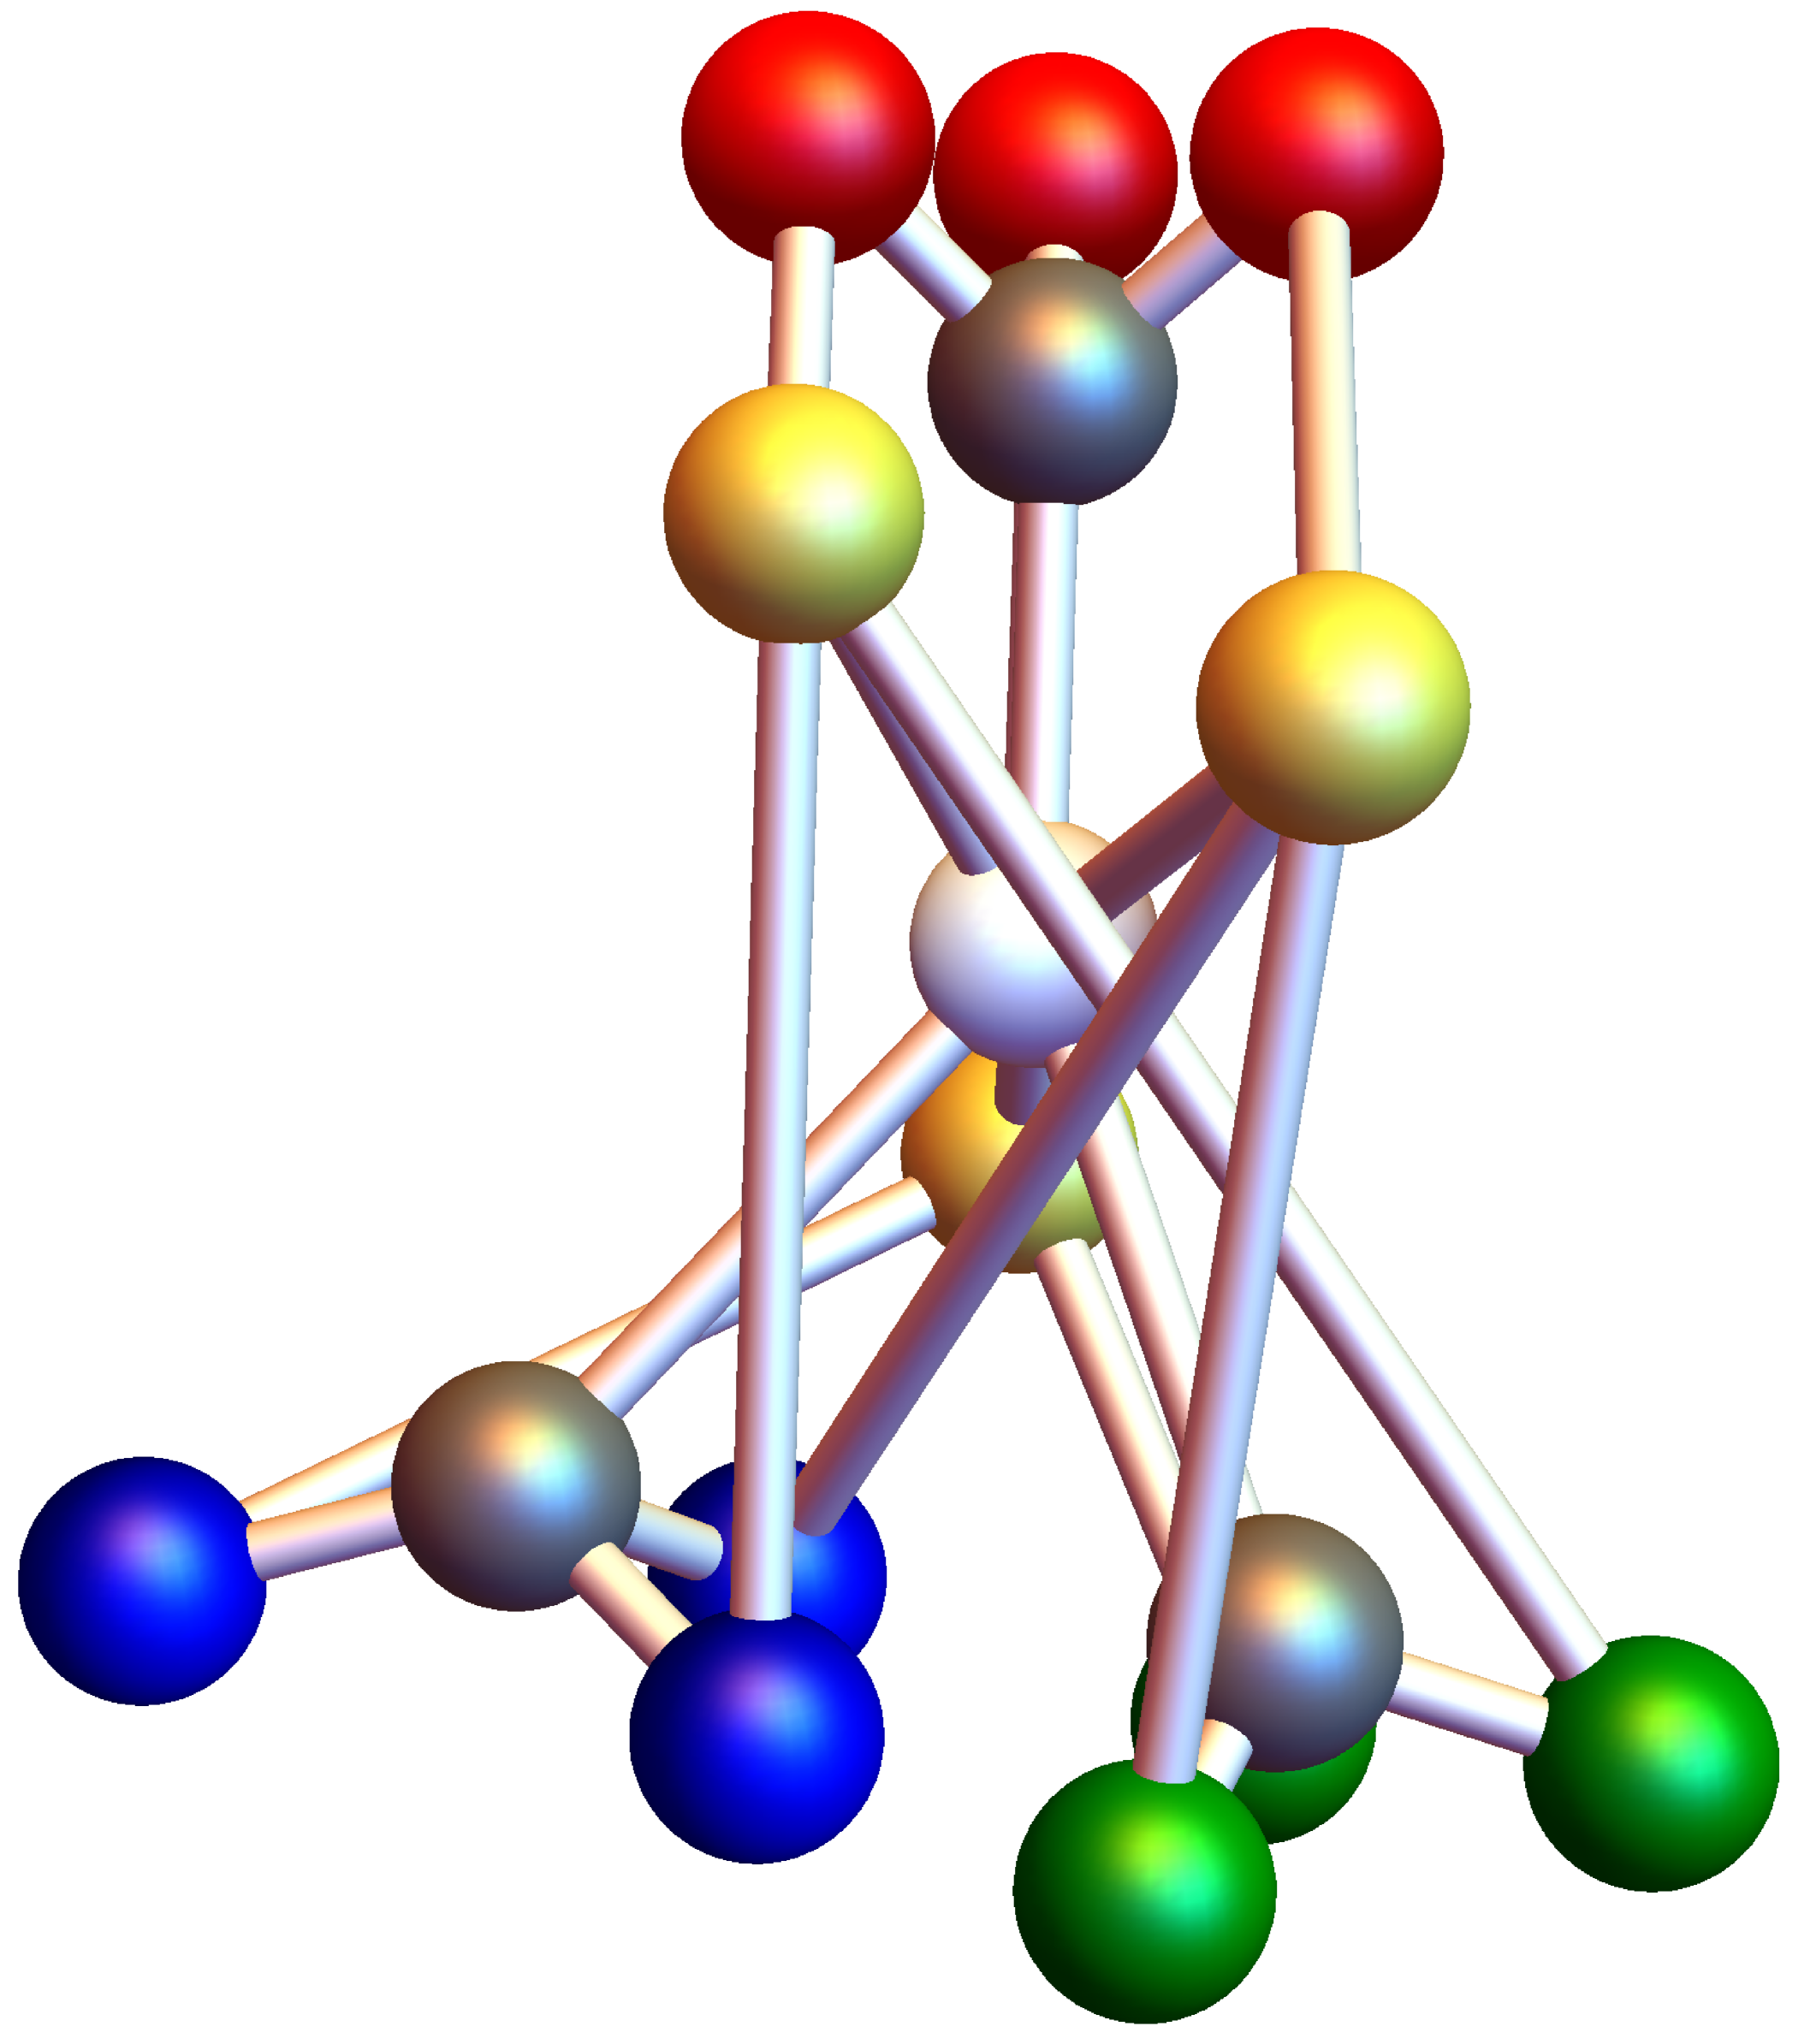
\includegraphics[trim=0mm 0 0 10mm, width=0.5\textwidth]{Images/switch_square.png} \\
			\vspace{0.4cm}
			\includegraphics[trim=0mm 0 0 10mm, width=0.8\textwidth]{Images/switchsquare-permutation}
		\end{center}
		\end{column}
	\end{columns}
\end{frame}}

\begin{center}
	\includeslide{routing1}
\end{center}

\noindent text


\mode<presentation>{\begin{frame}{Quantum Routing}\label{routing2}
	\begin{columns}[T]
		\begin{column}{0.5\textwidth}
		\begin{center}
			\includegraphics[trim=0mm 0 0 10mm, width=0.65\textwidth]{Images/switch_selfloops} \\
			\vspace{0.5cm}
			\includegraphics[trim=0mm 0 0 10mm, width=0.7\textwidth]{Images/switch2-permutation}
		\end{center}
		\end{column}
		\begin{column}{0.5\textwidth}
		\begin{center}
			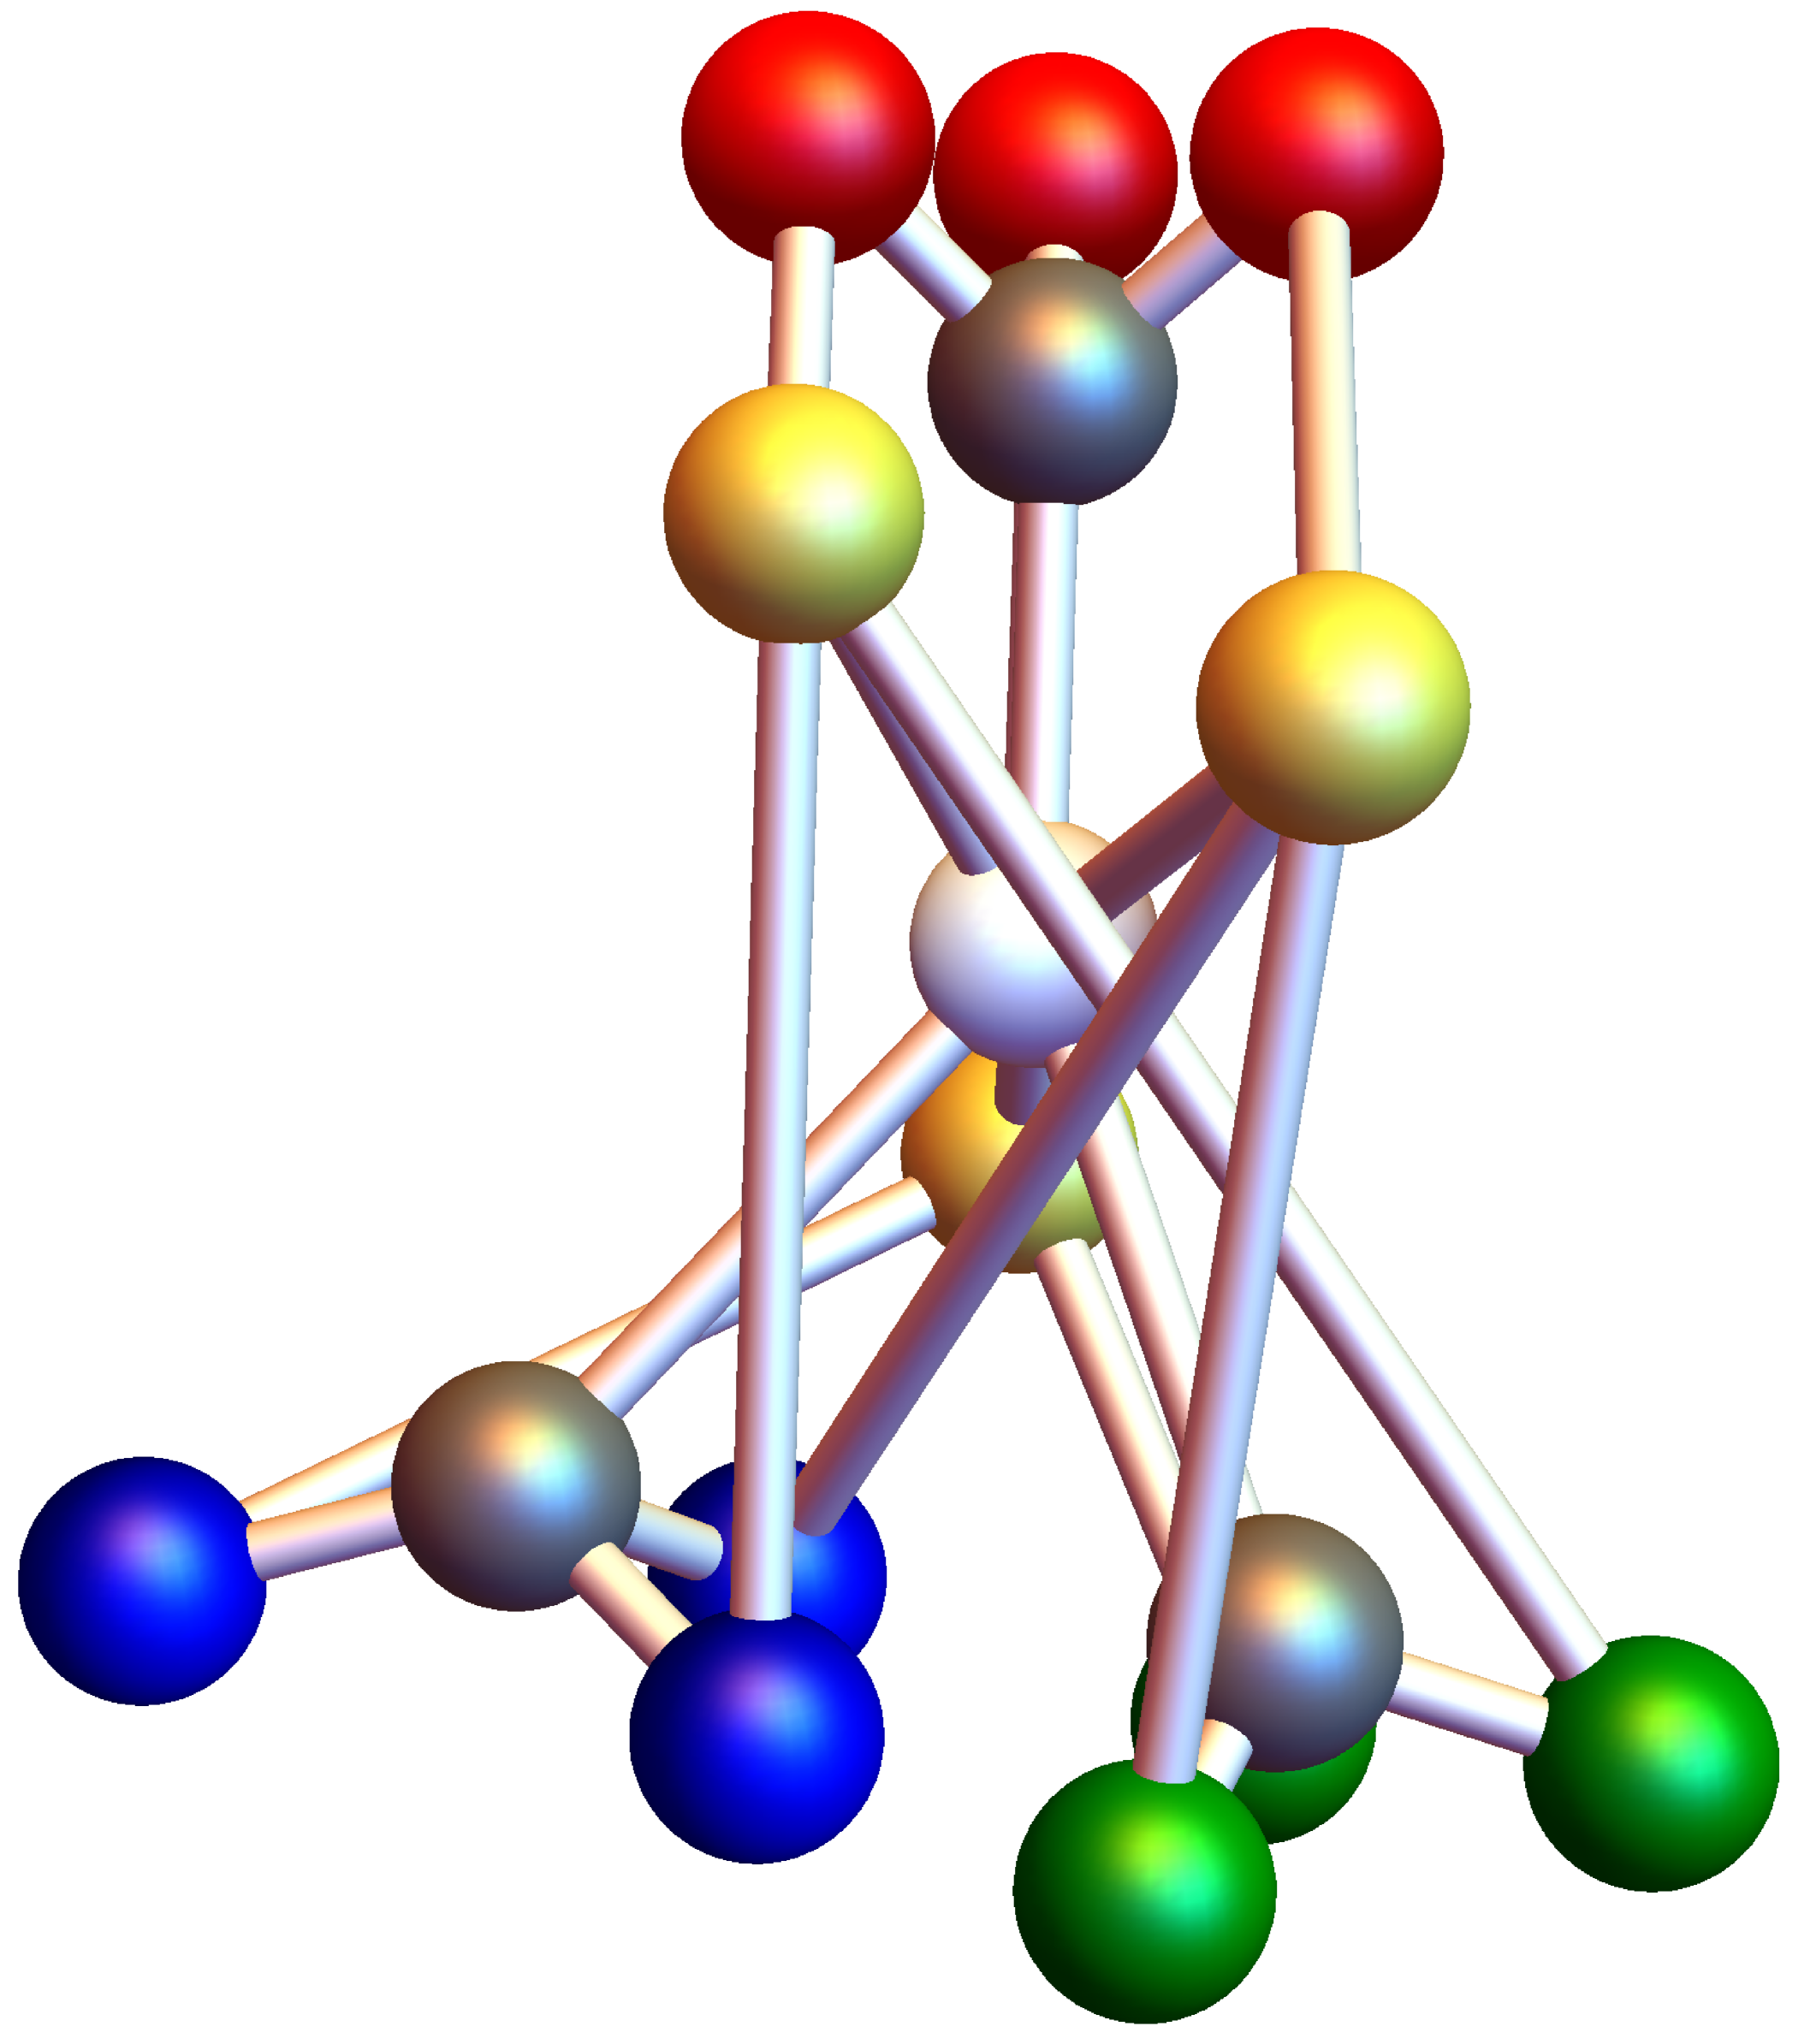
\includegraphics[trim=0mm 0 0 10mm, width=0.5\textwidth]{Images/switch_square.png} \\
			\vspace{0.4cm}
			\includegraphics[trim=0mm 0 0 10mm, width=0.8\textwidth]{Images/switchsquare2-permutation}
		\end{center}
		\end{column}
	\end{columns}
\end{frame}}

\begin{center}
	\includeslide{routing2}
\end{center}

\noindent text



\mode<presentation>{\begin{frame}{Higher Excitation Spaces}\label{hes}
	\begin{columns}[T]
		\begin{column}{0.5\textwidth}
		\begin{center}
			\includegraphics[trim=0mm 0 0 0mm, width=1.0\textwidth]{Images/method4-solution-chain2square} \\
			\includegraphics[trim=0mm 0 0 0mm, width=0.7\textwidth]{Images/chain2square-hes2-pst-marked}
		\end{center}
		\end{column}
		\begin{column}{0.5\textwidth}
		\begin{center}
			\includegraphics[trim=0mm 0 0 0mm, width=0.6\textwidth]{Images/chain2-cube} \\
			\includegraphics[trim=0mm 0 0 0mm, width=0.7\textwidth]{Images/chain2cube-hes2}
		\end{center}
		\end{column}
	\end{columns}
\end{frame}}

\begin{center}
	\includeslide{hes}
\end{center}

\noindent text


\mode<presentation>{\begin{frame}{Renormalization}\label{renormalization}
	\begin{columns}[T]
		\begin{column}{0.5\textwidth}
		\begin{center}
			\includegraphics[trim=0mm 0 0 0mm, width=1.0\textwidth]{Images/chain2-hypercube}
		\end{center}
		\end{column}
		\begin{column}{0.5\textwidth}
		\begin{center}
			\includegraphics[trim=0mm 0 0 0mm, width=1.0\textwidth]{Images/hypercube-to-perfect-couplings}
		\end{center}
		\end{column}
	\end{columns}
	\cite{Christandl2005}
\end{frame}}

\begin{center}
	\includeslide{renormalization}
\end{center}

\noindent text


\mode<presentation>{\begin{frame}{Renormalization}\label{renormalization2}	
	\begin{columns}[T]
		\begin{column}{0.5\textwidth}
		\begin{center}
			\includegraphics[trim=0mm 0 0 0mm, width=0.8\textwidth]{Images/eg-renorm-3}
		\end{center}
		\end{column}
		\begin{column}{0.5\textwidth}
		\begin{center}
			\includegraphics[trim=0mm 0 0 0mm, width=0.5\textwidth]{Images/eg-triplearmstar-uniform} \\
			\vspace*{0.3cm}
			\includegraphics[trim=0mm 0 0 0mm, width=0.45\textwidth]{Images/chain2square-hes2-pst-marked} \\
			\vspace*{0.3cm}
			\includegraphics[trim=0mm 0 0 0mm, width=0.5\textwidth]{Images/eg-pentaarmstar-uniform}
		\end{center}
		\end{column}
	\end{columns}
\end{frame}}

\begin{center}
	\includeslide{renormalization2}
\end{center}

\noindent text


\mode<presentation>{\begin{frame}{The Method}\label{method}
	\begin{columns}[T]
		\begin{column}{0.5\textwidth}
		\begin{center}
			\includegraphics[trim=0mm 0 0 0mm, width=0.65\textwidth]{Images/method7-graph}
		\end{center}
		\begin{align*}
	\begin{pmatrix}
		y_1 & y_2 & y_3 \\
		z_1 & z_2 & z_3 
	\end{pmatrix}
	\cdot
	\begin{pmatrix}
		a_1 & b_1 \\
		a_2 & b_2 \\
		a_3 & b_3 
	\end{pmatrix}
	\cdot
	\begin{pmatrix}
		1 \\
		0
	\end{pmatrix}
	&\mbeq
	\begin{pmatrix}
		1 \\
		0
	\end{pmatrix}
\end{align*}
		\end{column}
		\begin{column}{0.5\textwidth}
		\begin{center}
			\includegraphics[trim=0mm 0 0 0mm, width=0.5\textwidth]{Images/method7-solution-2chain3} \\
			\vspace*{0.8cm}
			\includegraphics[trim=0mm 0 0 0mm, width=0.45\textwidth]{Images/method7-solution-chain2square-hes2} \\
			%\vspace*{0.3cm}
			%\includegraphics[trim=0mm 0 0 0mm, width=0.5\textwidth]{Images/eg-pentaarmstar-uniform}
		\end{center}
		\end{column}
	\end{columns}

\end{frame}}

\begin{center}
	\includeslide{method}
\end{center}

\noindent text


\mode<presentation>{\begin{frame}{Conclusion}\label{conclusion}
	\begin{itemize}
		\item Designing networks for defined system topologies is possible 
		\item If these networks are realizable is questionable
		\item Some classical algorithms may be impossible to implement on QC
	\end{itemize}
\end{frame}}

\begin{center}
	\includeslide{conclusion}
\end{center}

\noindent text



\end{document}
